\chapter{MÓDULOS E FUNCIONALIDADES DO FRONTEND}

Este capítulo apresenta a estrutura funcional da interface do usuário (UI) do sistema de Registro de Ponto. A aplicação foi desenvolvida com o framework Next.js e segue uma arquitetura modular, onde cada responsabilidade principal do sistema é encapsulada em uma seção específica. A seguir, são detalhados os principais módulos e suas respectivas funcionalidades, demonstrando como a solução atende aos requisitos de um sistema de gestão de ponto moderno e eficiente.

\section{Autenticação de Usuários}

O primeiro contato do usuário com o sistema ocorre através da tela de autenticação. A interface de login, de design minimalista, solicita as credenciais do usuário (e-mail e senha) para garantir o acesso seguro à plataforma.

\begin{figure}[H]
\centering
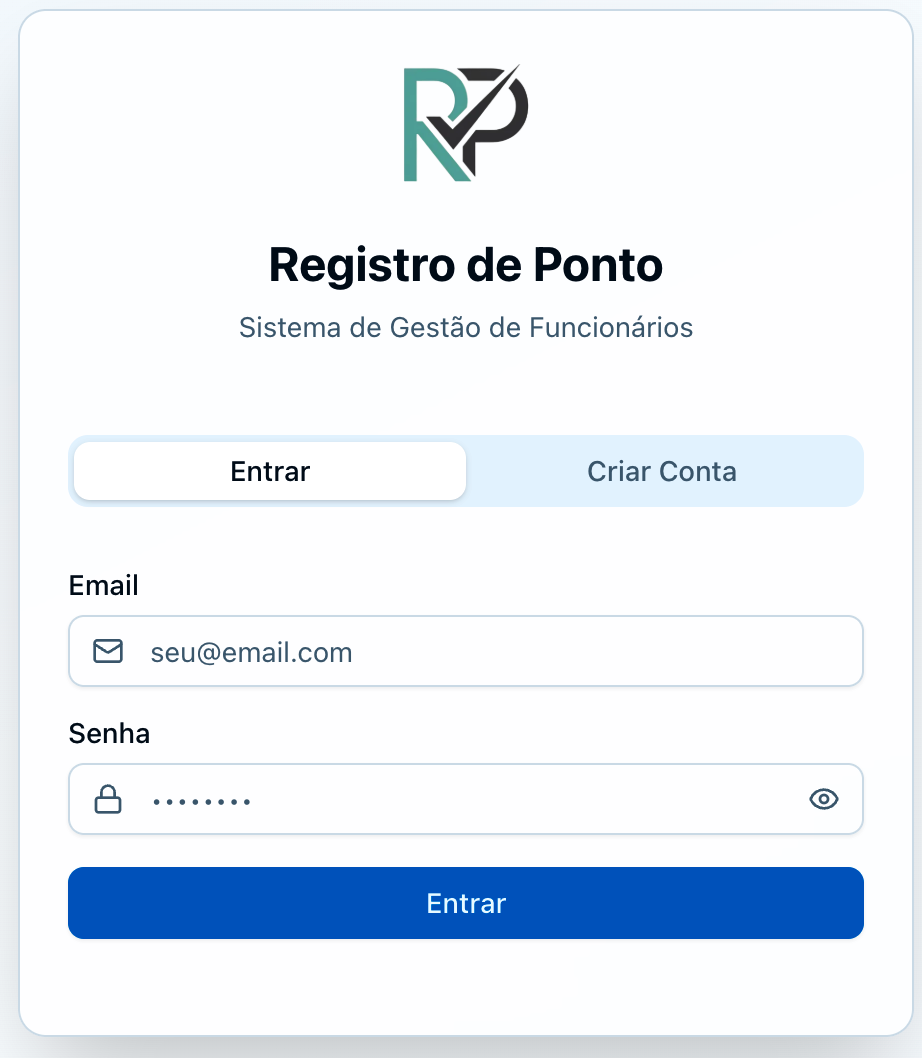
\includegraphics[width=0.5\textwidth]{imagens/tela-login.png}
\caption{Tela de login do sistema}
\label{fig:tela-login}
\end{figure}

\section{Painel Principal (Dashboard)}

Após a autenticação bem-sucedida, o usuário é direcionado ao Dashboard, que serve como uma central de informações e navegação. Esta tela apresenta uma visão geral e consolidada dos dados mais relevantes da operação, permitindo que o gestor tenha um panorama rápido da situação atual da equipe. O painel é composto por:

\begin{itemize}
\item \textbf{Cards de Métricas}: Exibem indicadores chave, como o total de funcionários ativos, a média de horas trabalhadas e o número de faltas no período.
\item \textbf{Gráfico de Assiduidade}: Um gráfico de barras que ilustra a frequência de registros de ponto ao longo da semana, permitindo identificar padrões de assiduidade.
\item \textbf{Atividades Recentes}: Uma lista com os últimos registros de ponto e justificativas enviadas, oferecendo um acompanhamento em tempo real.
\end{itemize}

\begin{figure}[H]
\centering
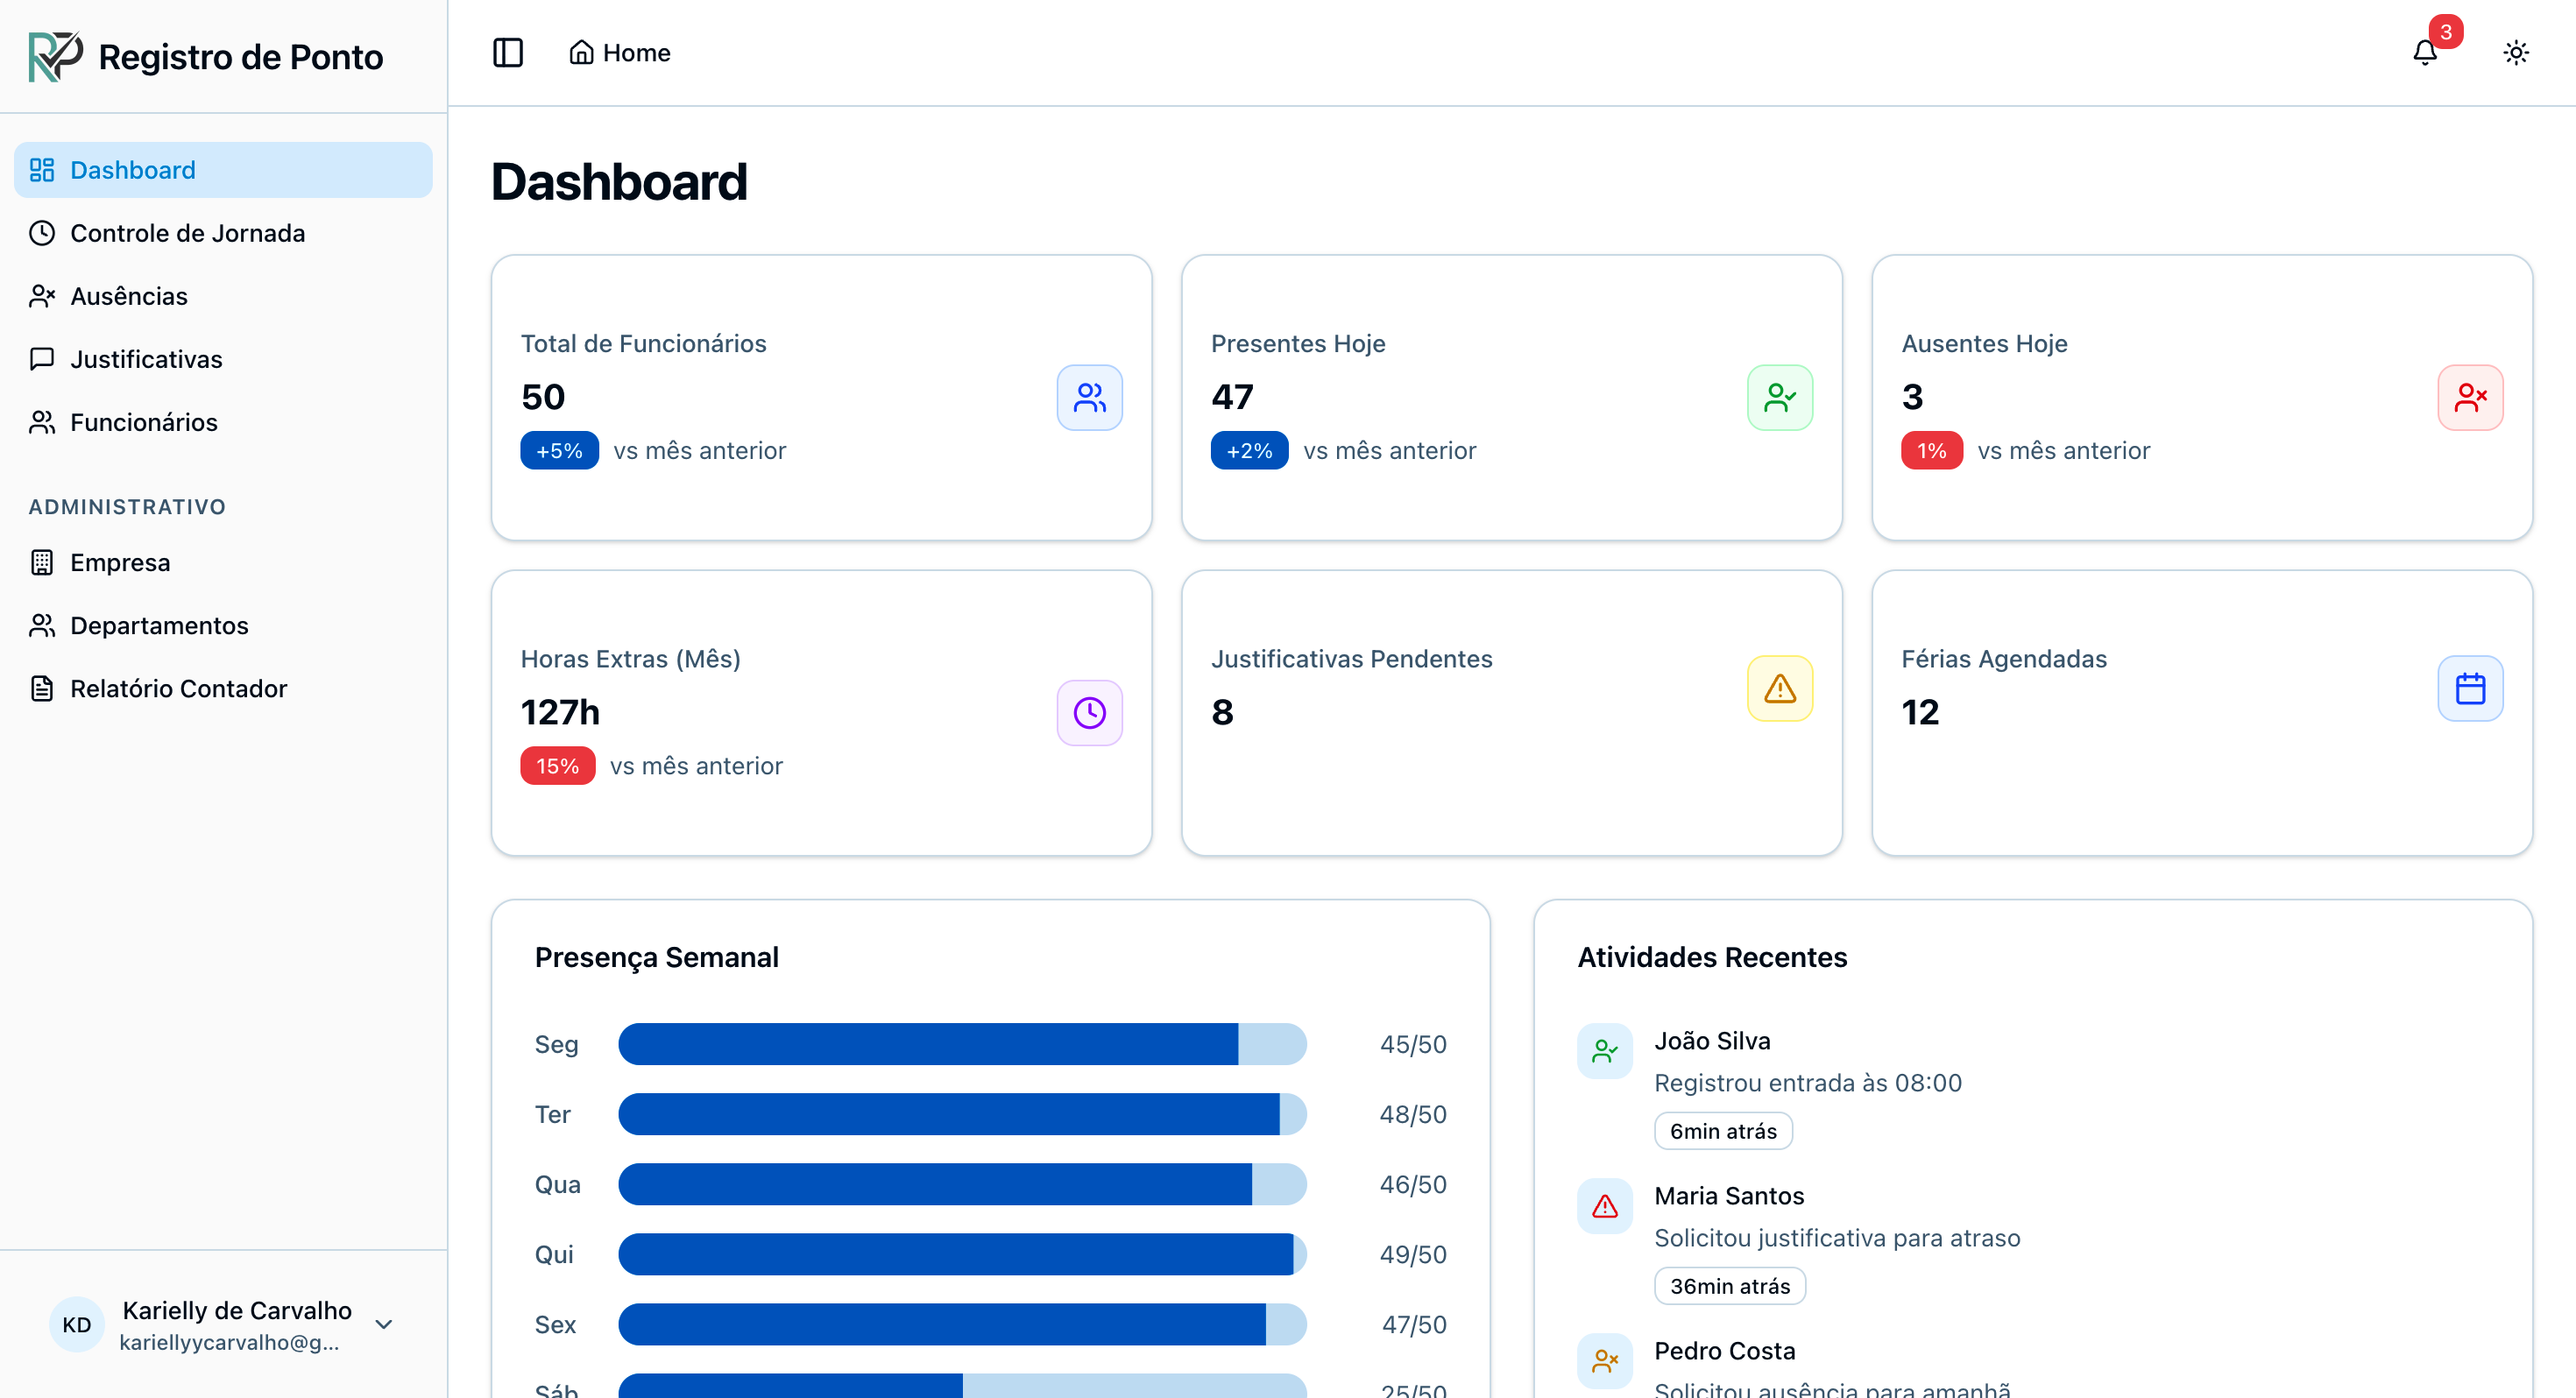
\includegraphics[width=0.7\textwidth]{imagens/dashboard-principal.png}
\caption{Dashboard principal com métricas e visão geral}
\label{fig:dashboard-principal}
\end{figure}

\section{Módulo de Funcionários}

Este é um dos módulos centrais do sistema, dedicado ao gerenciamento completo do cadastro dos colaboradores da empresa. A tela principal exibe uma tabela com a lista de todos os funcionários, permitindo buscas e filtros.

\begin{figure}[H]
\centering
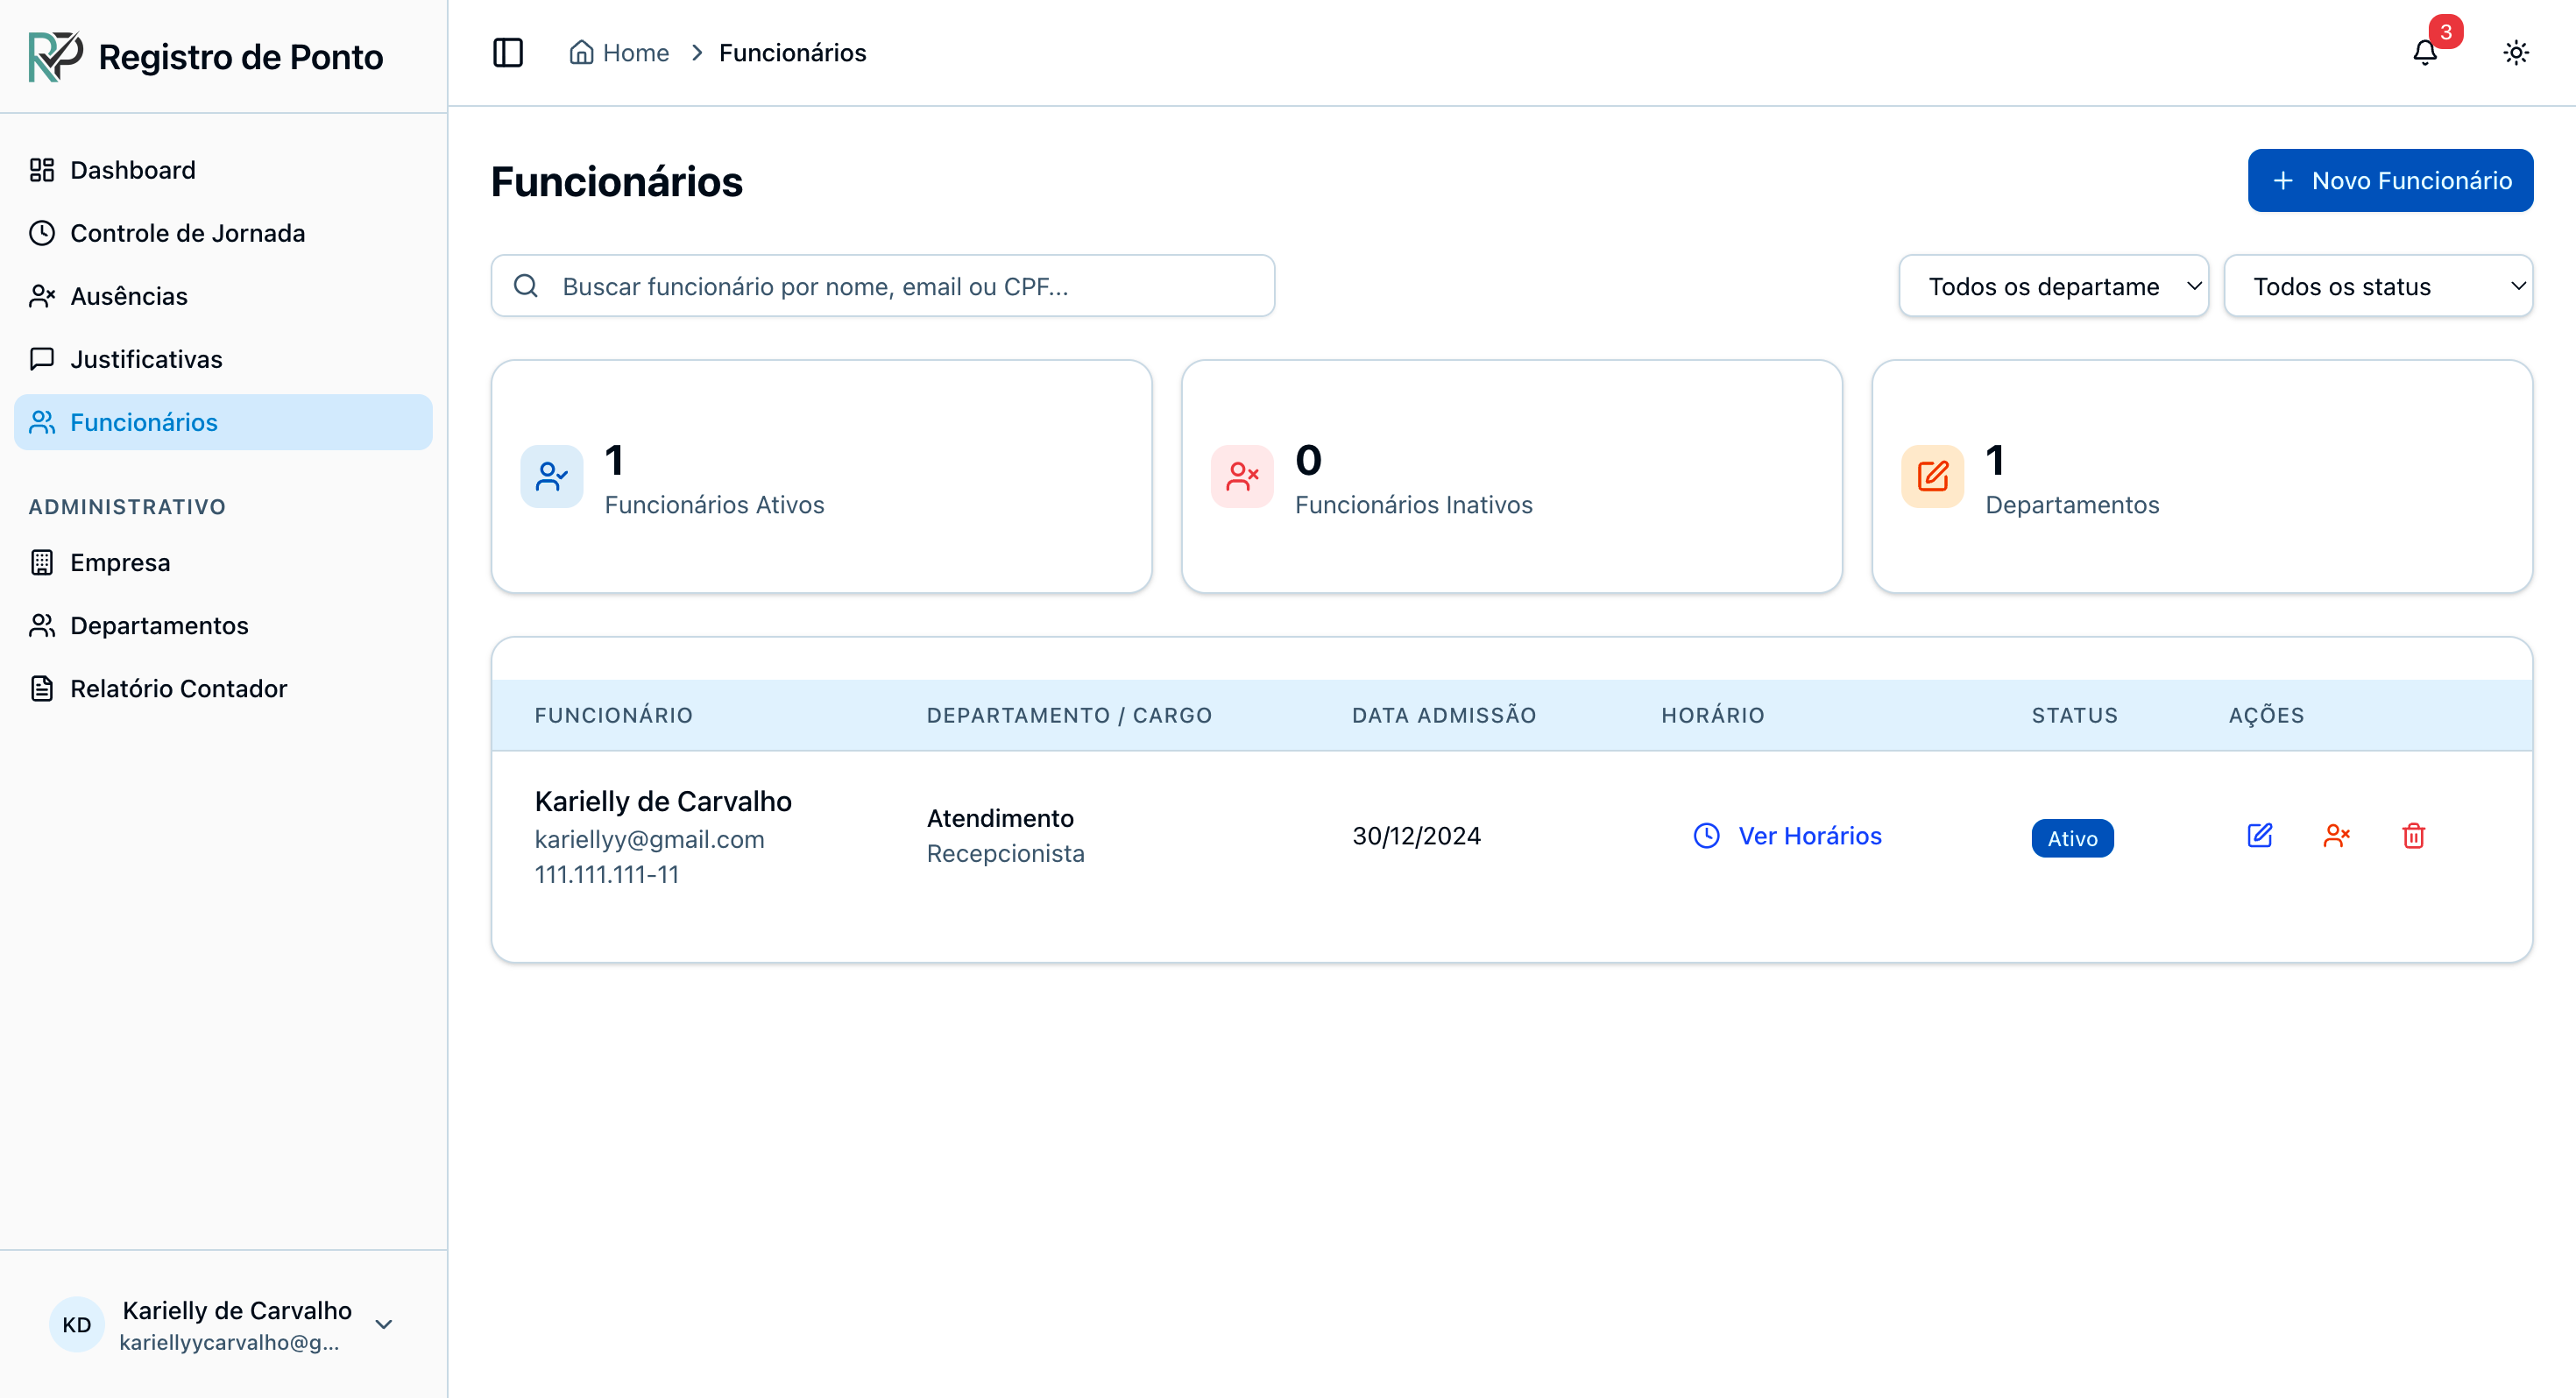
\includegraphics[width=0.7\textwidth]{imagens/listagem-funcionarios.png}
\caption{Tela de listagem e gerenciamento de funcionários}
\label{fig:listagem-funcionarios}
\end{figure}

As principais funcionalidades deste módulo são:

\begin{itemize}
\item \textbf{Cadastro de Novo Funcionário}: Através de um modal, o gestor pode adicionar novos colaboradores, inserindo informações pessoais, dados contratuais e associando-os a um departamento e a uma jornada de trabalho específica.
\item \textbf{Edição e Visualização}: Cada funcionário na lista possui ações para editar suas informações ou visualizar seus detalhes em uma página dedicada.
\item \textbf{Gestão de Horários Individuais}: O sistema permite a configuração de horários de trabalho específicos para cada funcionário, oferecendo flexibilidade para diferentes regimes de trabalho.
\end{itemize}

\section{Módulo de Departamentos}

Para organizar a estrutura da empresa, o sistema conta com um módulo para a gestão de departamentos. A interface permite que o administrador crie, renomeie e exclua os departamentos aos quais os funcionários serão vinculados.

\begin{figure}[H]
\centering
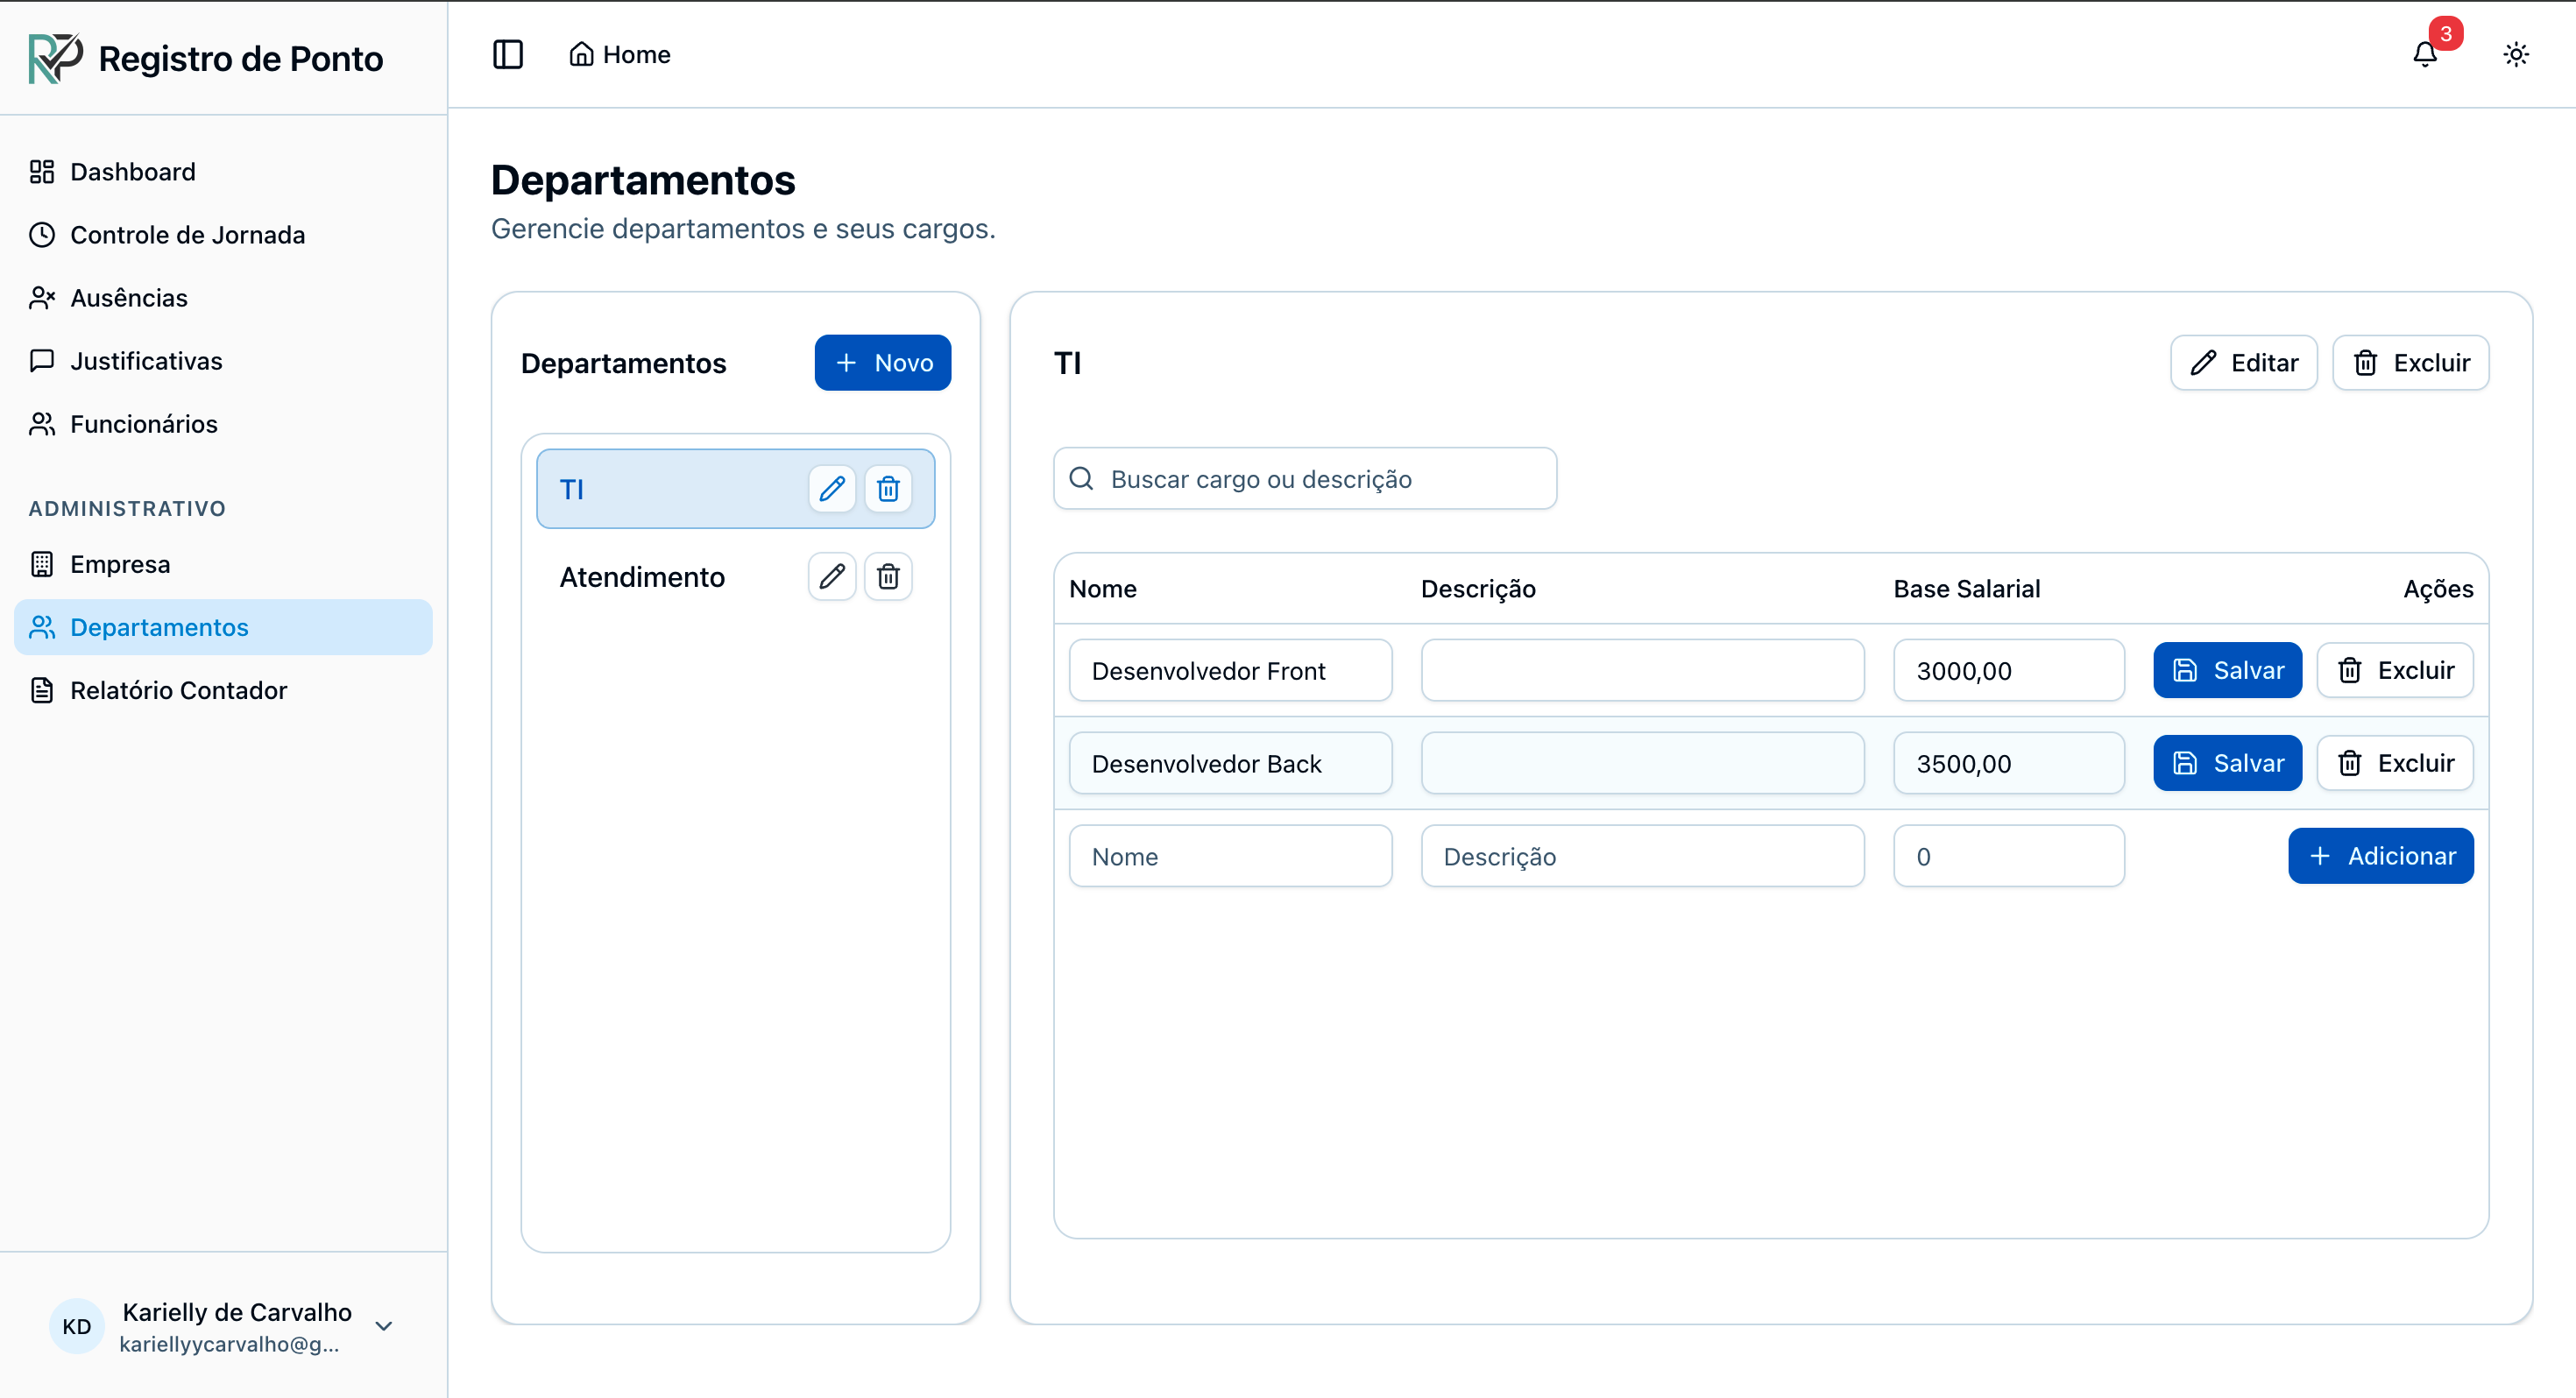
\includegraphics[width=0.7\textwidth]{imagens/gestao-departamentos.png}
\caption{Tela de gestão de departamentos}
\label{fig:gestao-departamentos}
\end{figure}

\section{Módulo de Jornada de Trabalho}

Esta seção permite a criação e configuração dos diferentes regimes de jornada de trabalho praticados pela empresa. O gestor pode definir os horários padrão de entrada, saída e intervalos para cada dia da semana. Essas jornadas pré-configuradas podem ser posteriormente associadas aos funcionários, padronizando os horários e facilitando a gestão.

\begin{figure}[H]
\centering
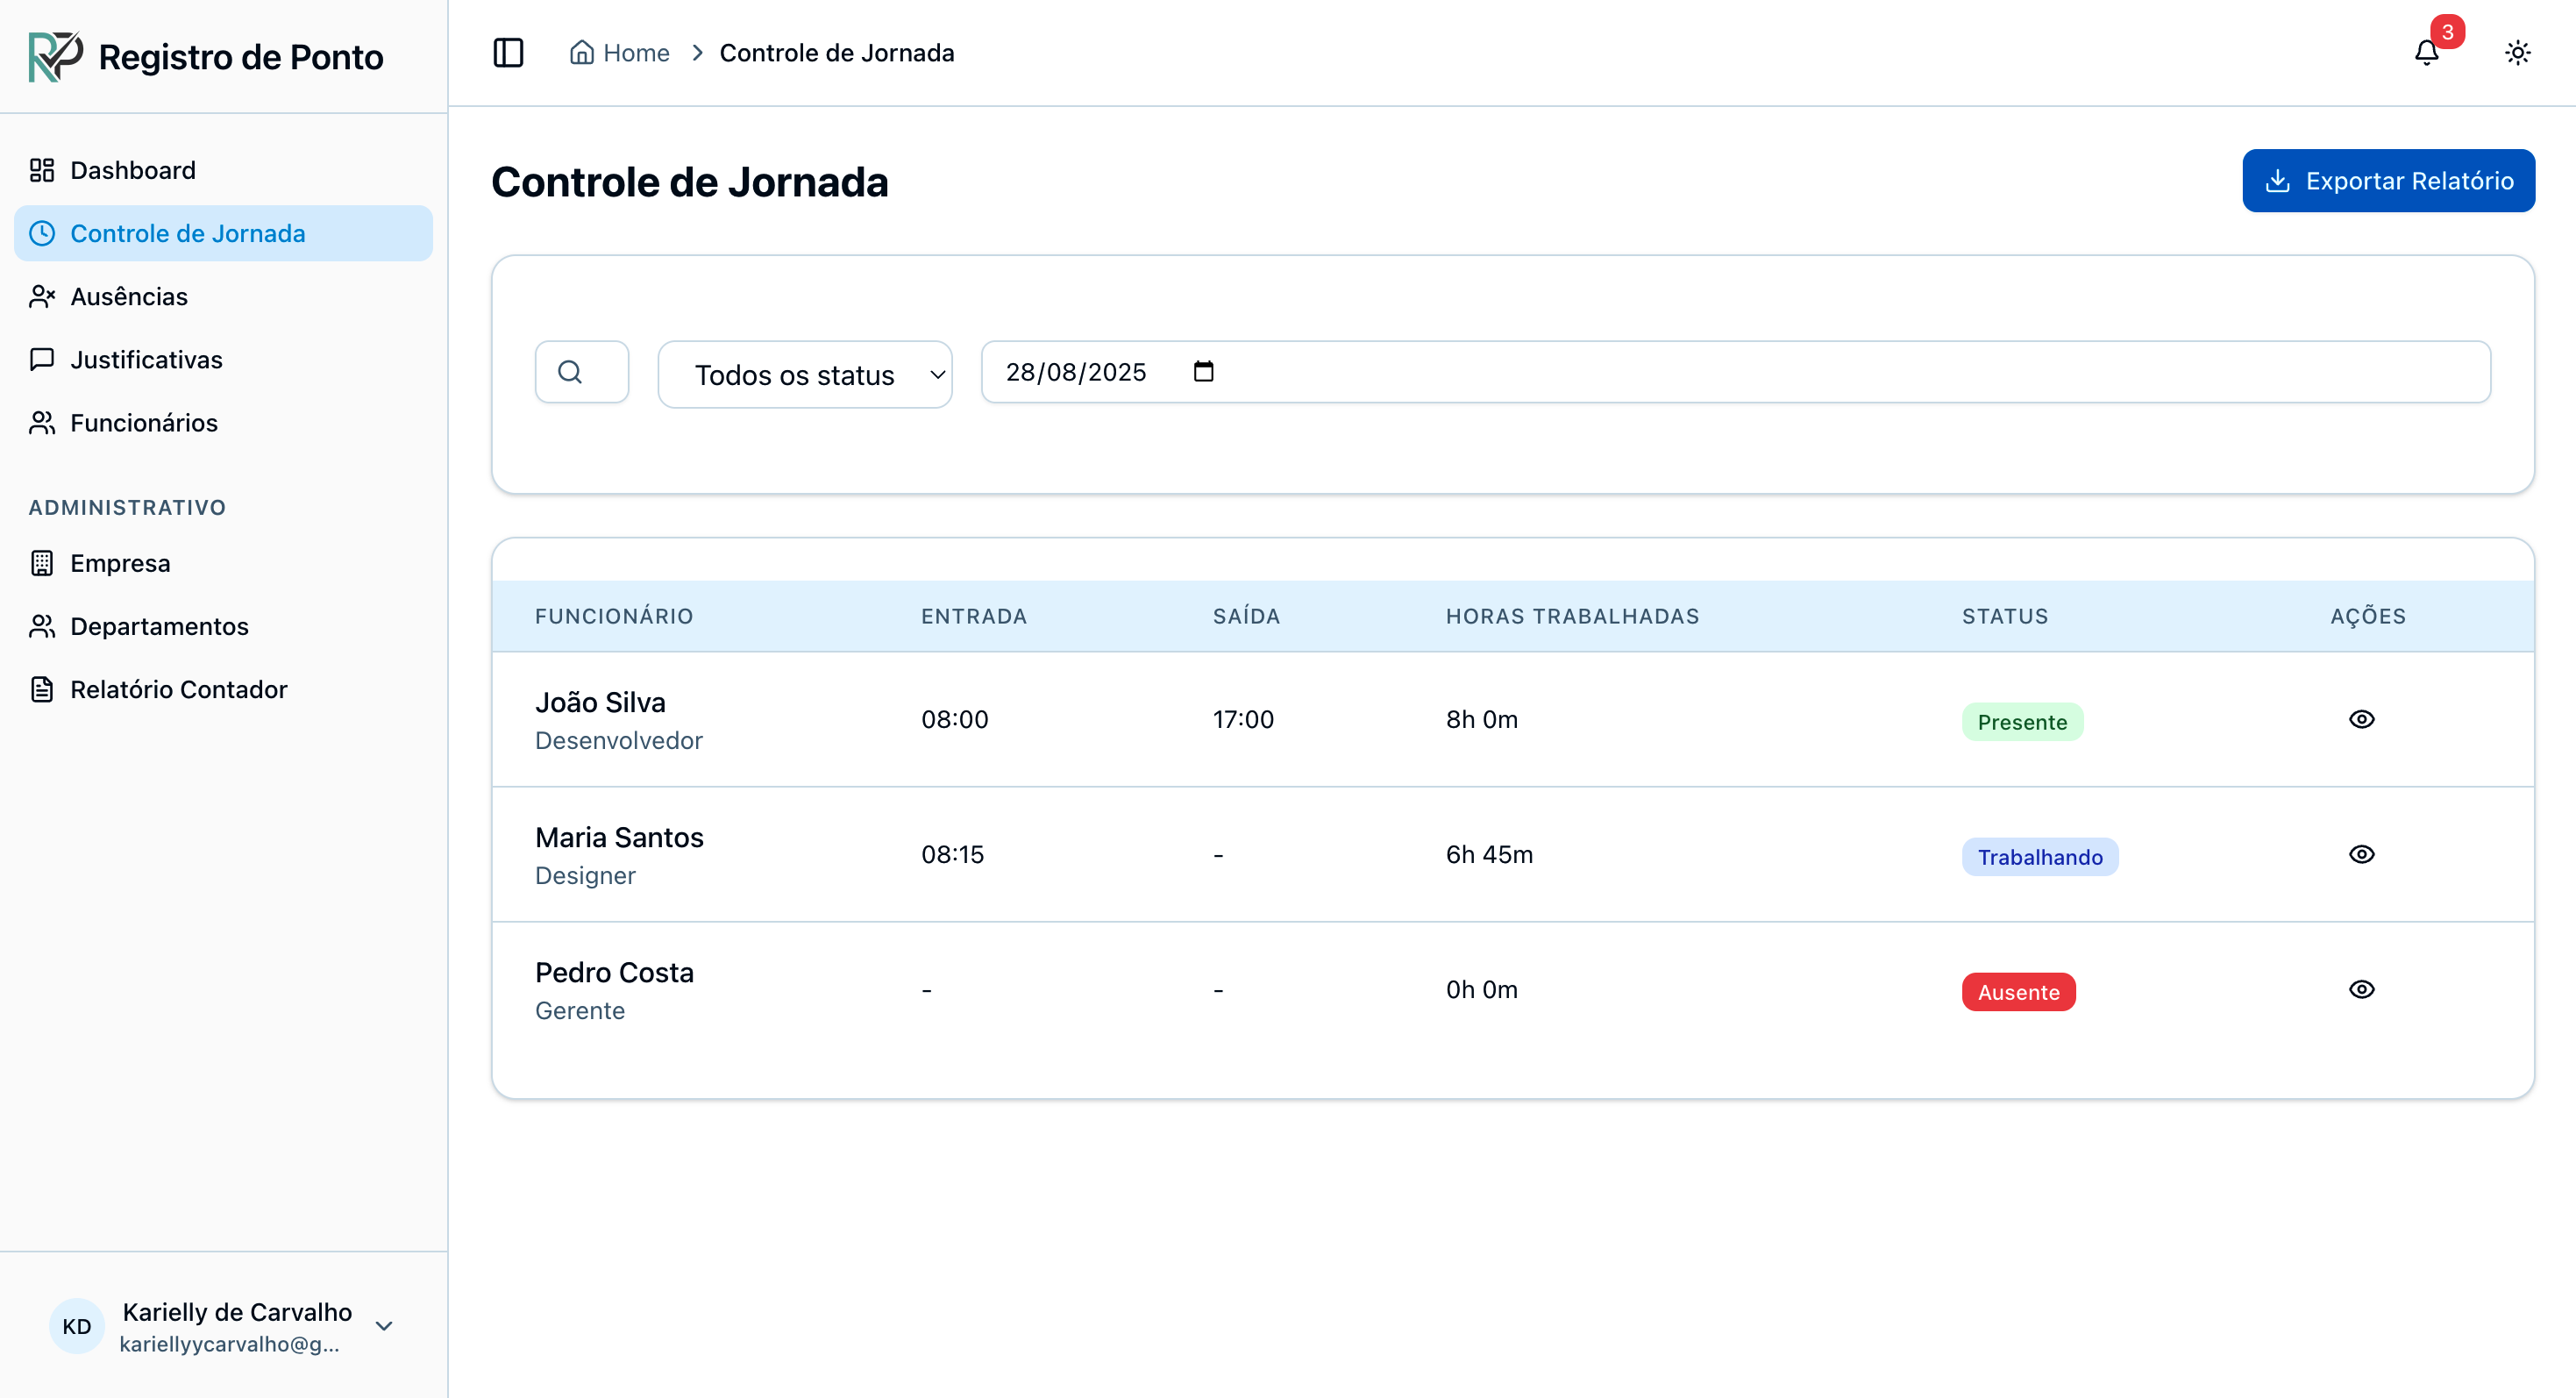
\includegraphics[width=0.7\textwidth]{imagens/configuracao-jornada.png}
\caption{Configuração de jornadas de trabalho}
\label{fig:configuracao-jornada}
\end{figure}

\section{Módulo de Justificativas}

Este módulo centraliza a gestão de ausências e atrasos. A interface permite que os gestores analisem as justificativas enviadas pelos funcionários, que podem incluir anexos como atestados médicos.

\begin{figure}[H]
\centering
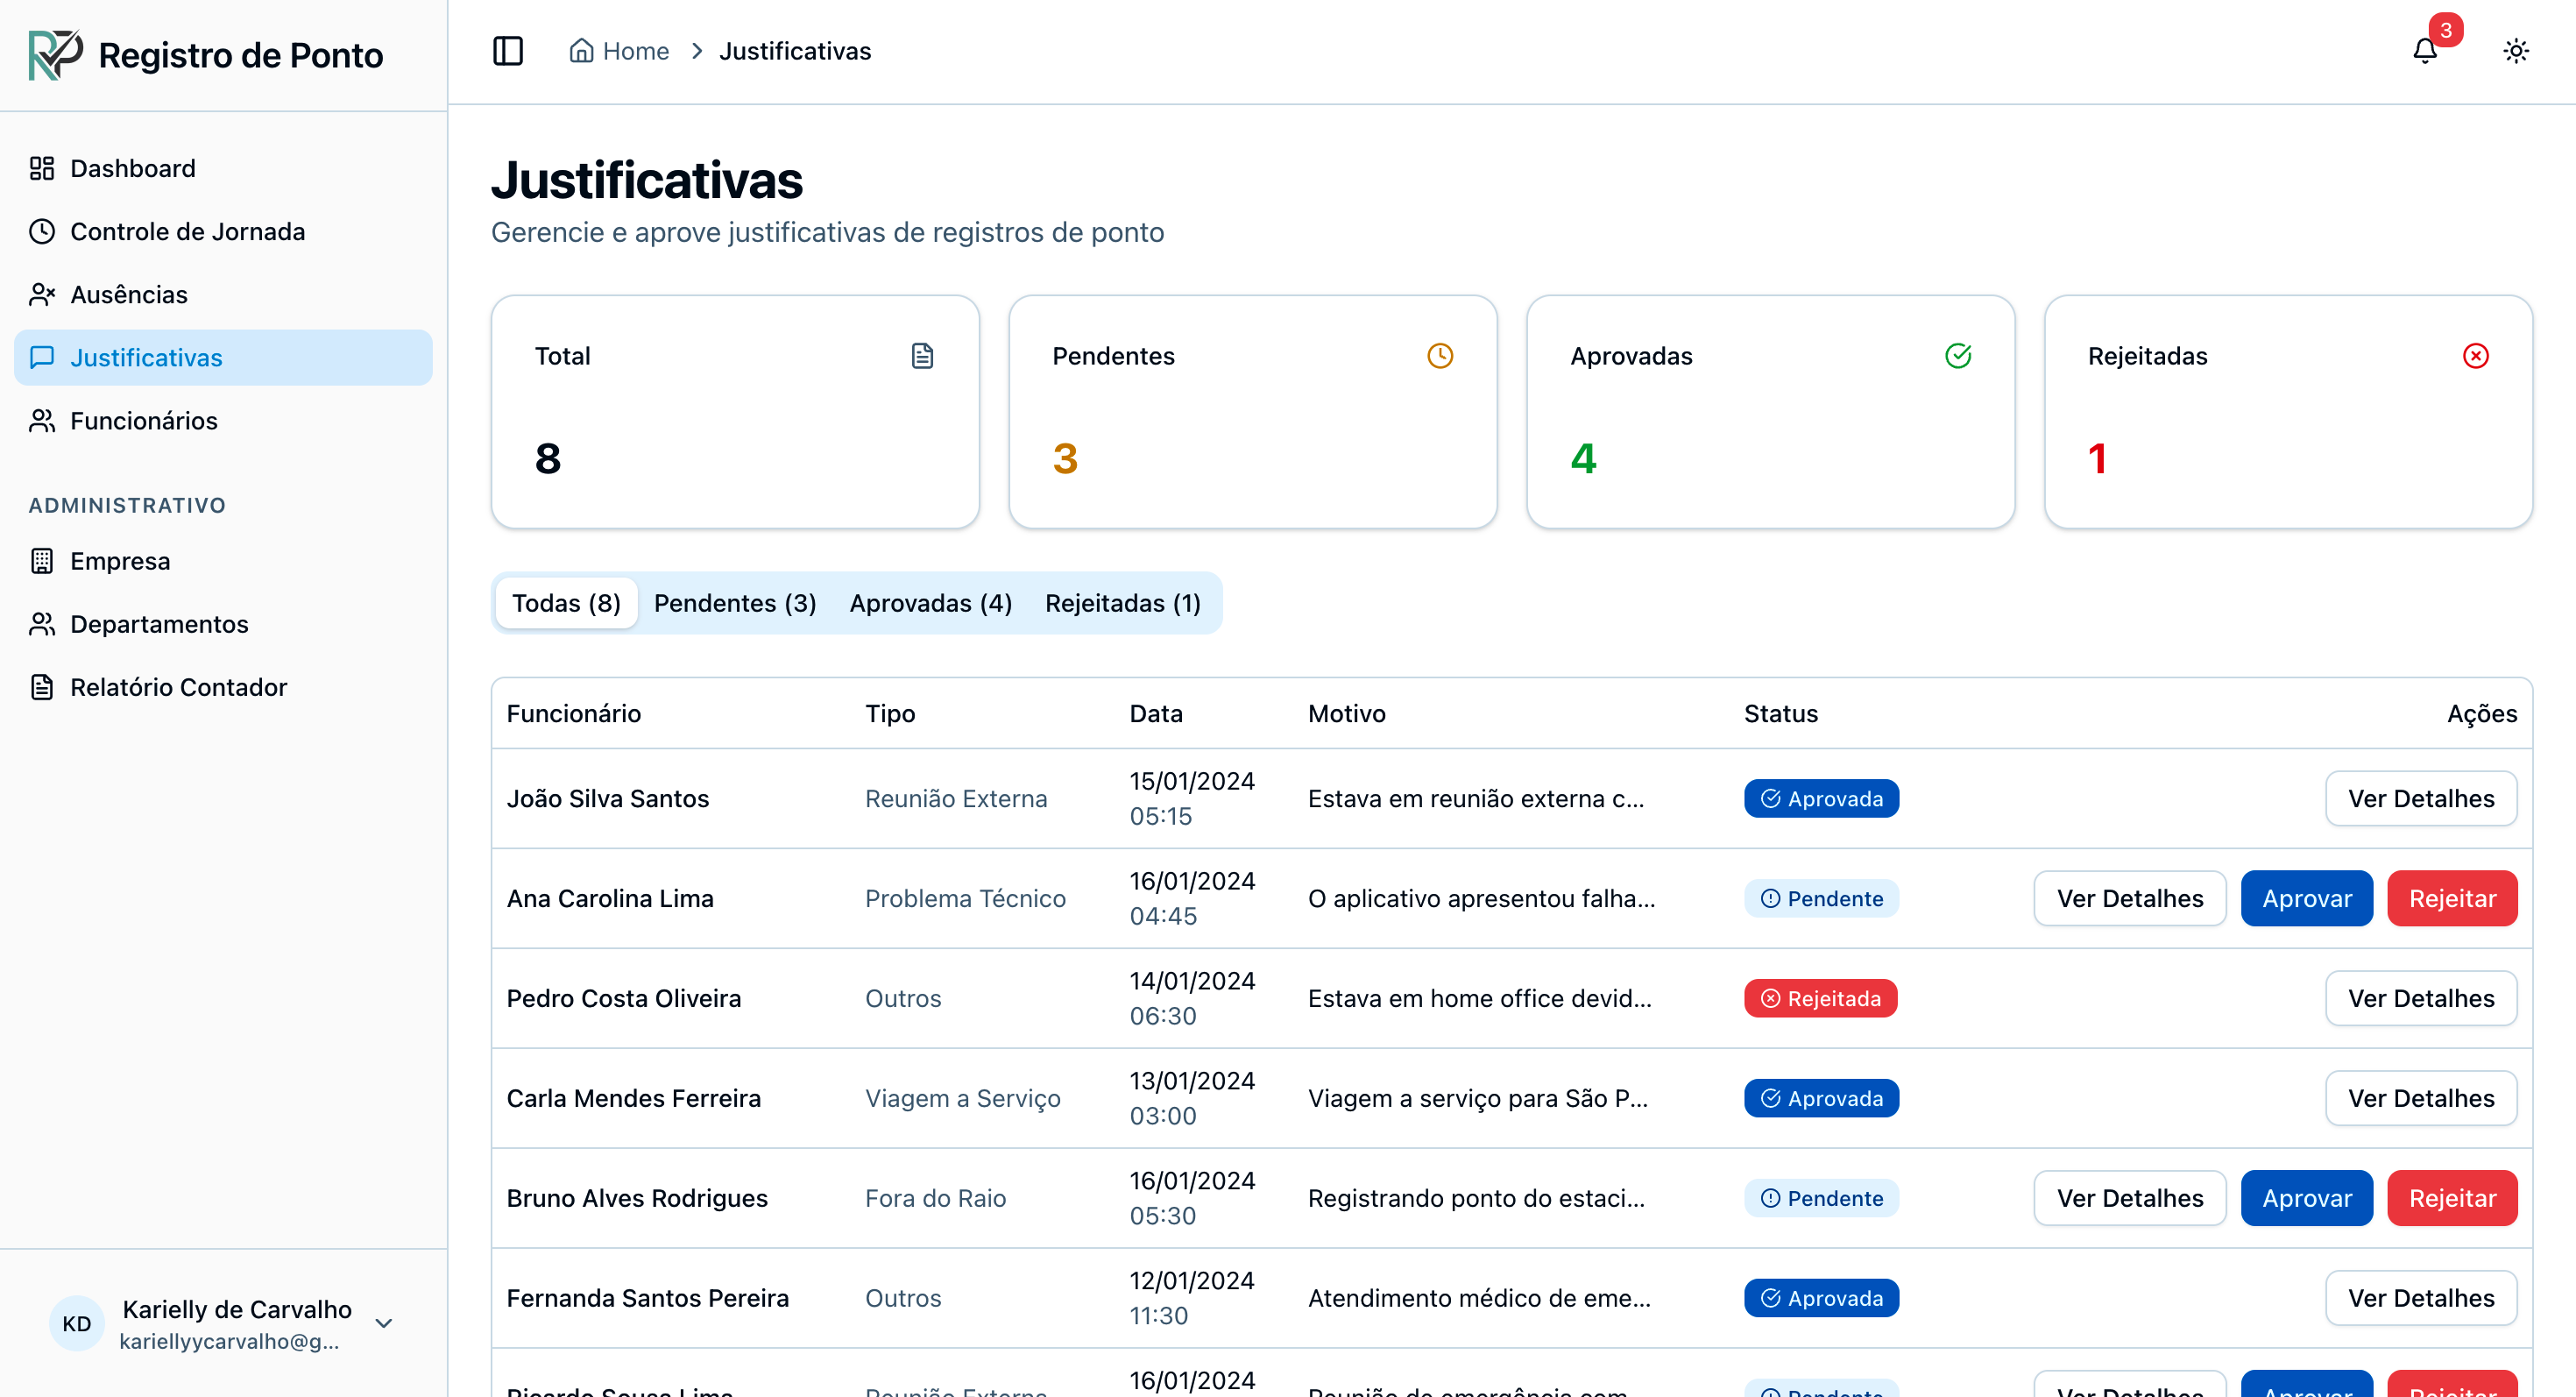
\includegraphics[width=0.7\textwidth]{imagens/gestao-justificativas.png}
\caption{Tela de gestão de justificativas}
\label{fig:gestao-justificativas}
\end{figure}

O fluxo de aprovação é simples e direto: o gestor pode visualizar os detalhes de cada justificativa, incluindo o anexo, e optar por "Aprovar" ou "Recusar" a solicitação através de um modal de confirmação, garantindo a rastreabilidade das decisões.

\section{Módulo de Controle de Ausências}

Complementando o módulo de justificativas, o sistema oferece uma interface específica para o controle detalhado de ausências. Esta tela permite o registro e acompanhamento de diferentes tipos de ausências como atestados médicos, licenças e faltas não justificadas.

\begin{figure}[H]
\centering
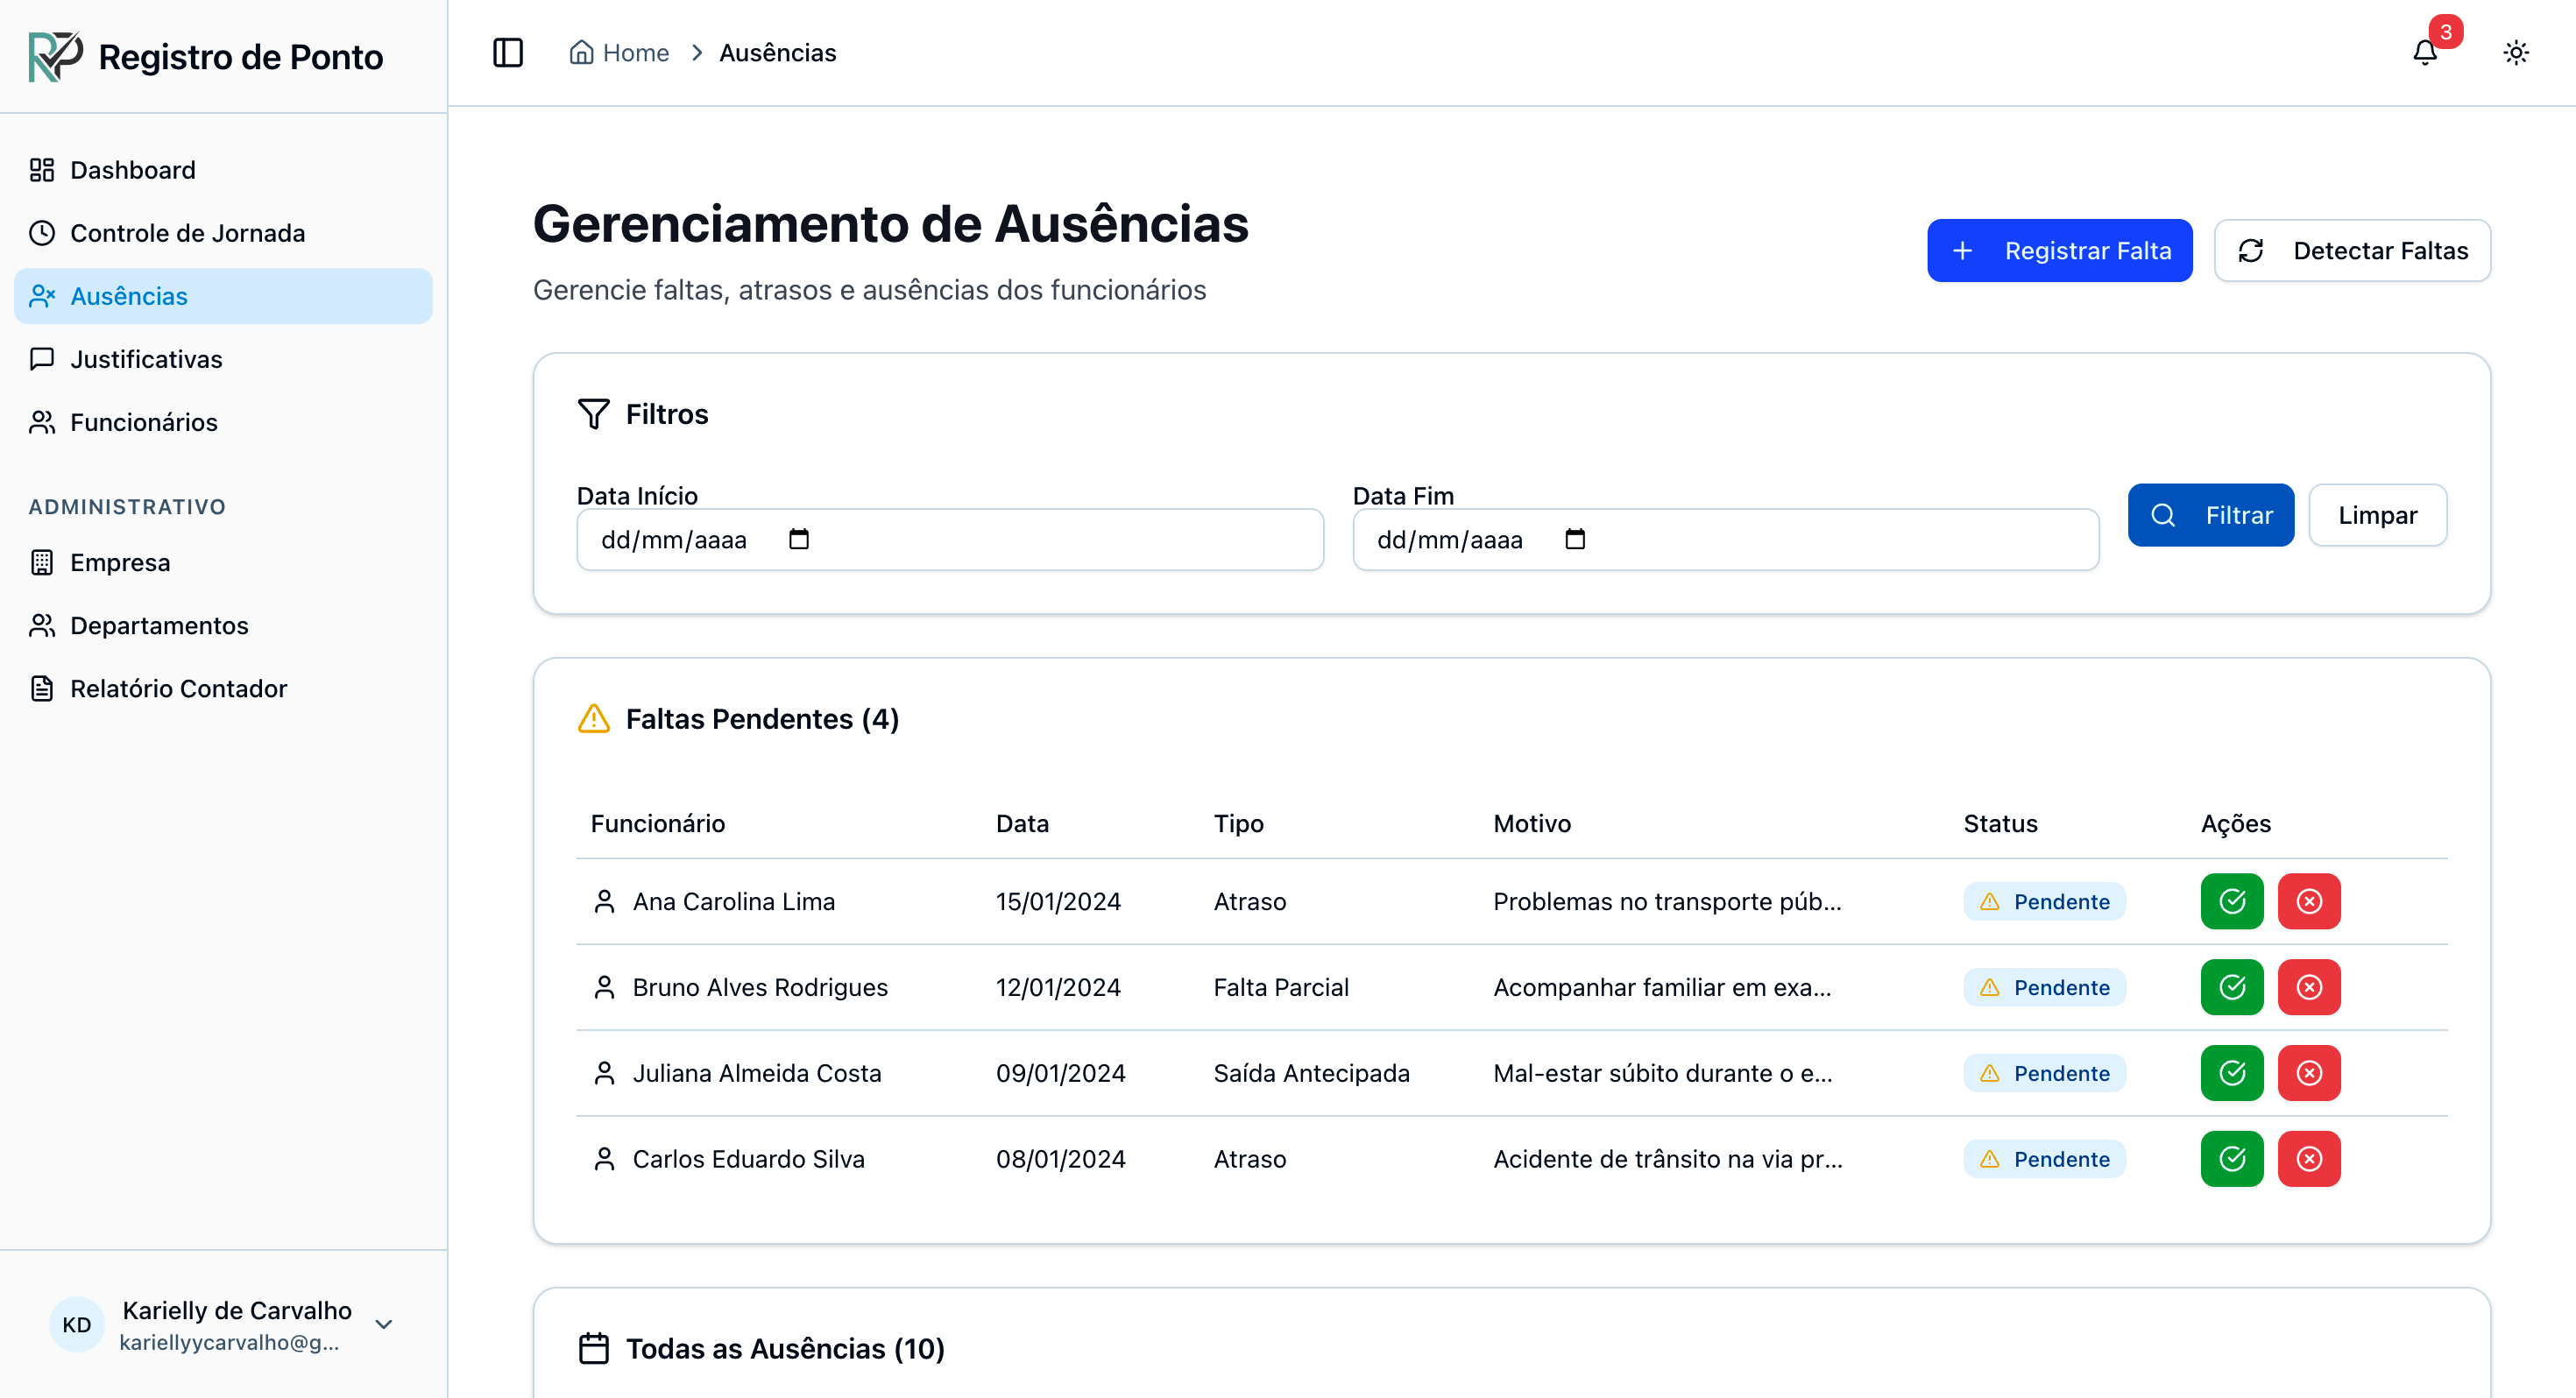
\includegraphics[width=0.7\textwidth]{imagens/controle-ausencias.png}
\caption{Controle detalhado de ausências por tipo}
\label{fig:controle-ausencias}
\end{figure}

As funcionalidades incluem:

\begin{itemize}
\item \textbf{Classificação por Tipo}: Separação entre atestados médicos, licenças, faltas e feriados.
\item \textbf{Controle de Status}: Visualização do status de aprovação (pendente, aprovada, rejeitada).
\item \textbf{Filtros Avançados}: Busca por funcionário, tipo de ausência e status.
\item \textbf{Registro de Período}: Controle de data início, fim e total de dias da ausência.
\end{itemize}

\section{Módulo de Gestão de Férias}

O sistema disponibiliza um módulo completo para gestão de férias, permitindo o controle dos períodos aquisitivos, saldos disponíveis e agendamento de períodos de descanso.

\begin{figure}[H]
\centering
\includegraphics[width=0.7\textwidth]{imagens/gestao-ferias.png}
\caption{Gestão completa de férias e períodos aquisitivos}
\label{fig:gestao-ferias}
\end{figure}

O módulo apresenta:

\begin{itemize}
\item \textbf{Controle de Períodos Aquisitivos}: Acompanhamento dos períodos de direito a férias.
\item \textbf{Saldo de Dias}: Visualização de dias de direito, usados e restantes.
\item \textbf{Agendamento}: Interface para agendar próximos períodos de férias.
\item \textbf{Resumo Estatístico}: Visão geral com métricas de toda a equipe.
\end{itemize}

\section{Módulo de Relatórios}

\subsection{Extrato de Ponto}

A plataforma oferece uma interface dedicada à geração de relatórios, essencial para o fechamento da folha de pagamento. A tela "Extrato de Ponto" permite ao gestor ou ao contador filtrar os registros de um funcionário específico dentro de um período de datas.

\begin{figure}[H]
\centering
\includegraphics[width=0.7\textwidth]{imagens/extrato-ponto.png}
\caption{Tela de extrato de ponto individual}
\label{fig:extrato-ponto}
\end{figure}

O sistema exibe uma tabela detalhada com todos os registros de entrada e saída do colaborador no período selecionado, calculando o saldo de horas e permitindo a exportação dos dados para análise externa.

\subsection{Relatório para Contador}

Para facilitar o trabalho contábil, o sistema oferece uma interface específica que consolida informações mensais de todos os funcionários em formato adequado para processamento da folha de pagamento.

\begin{figure}[H]
\centering
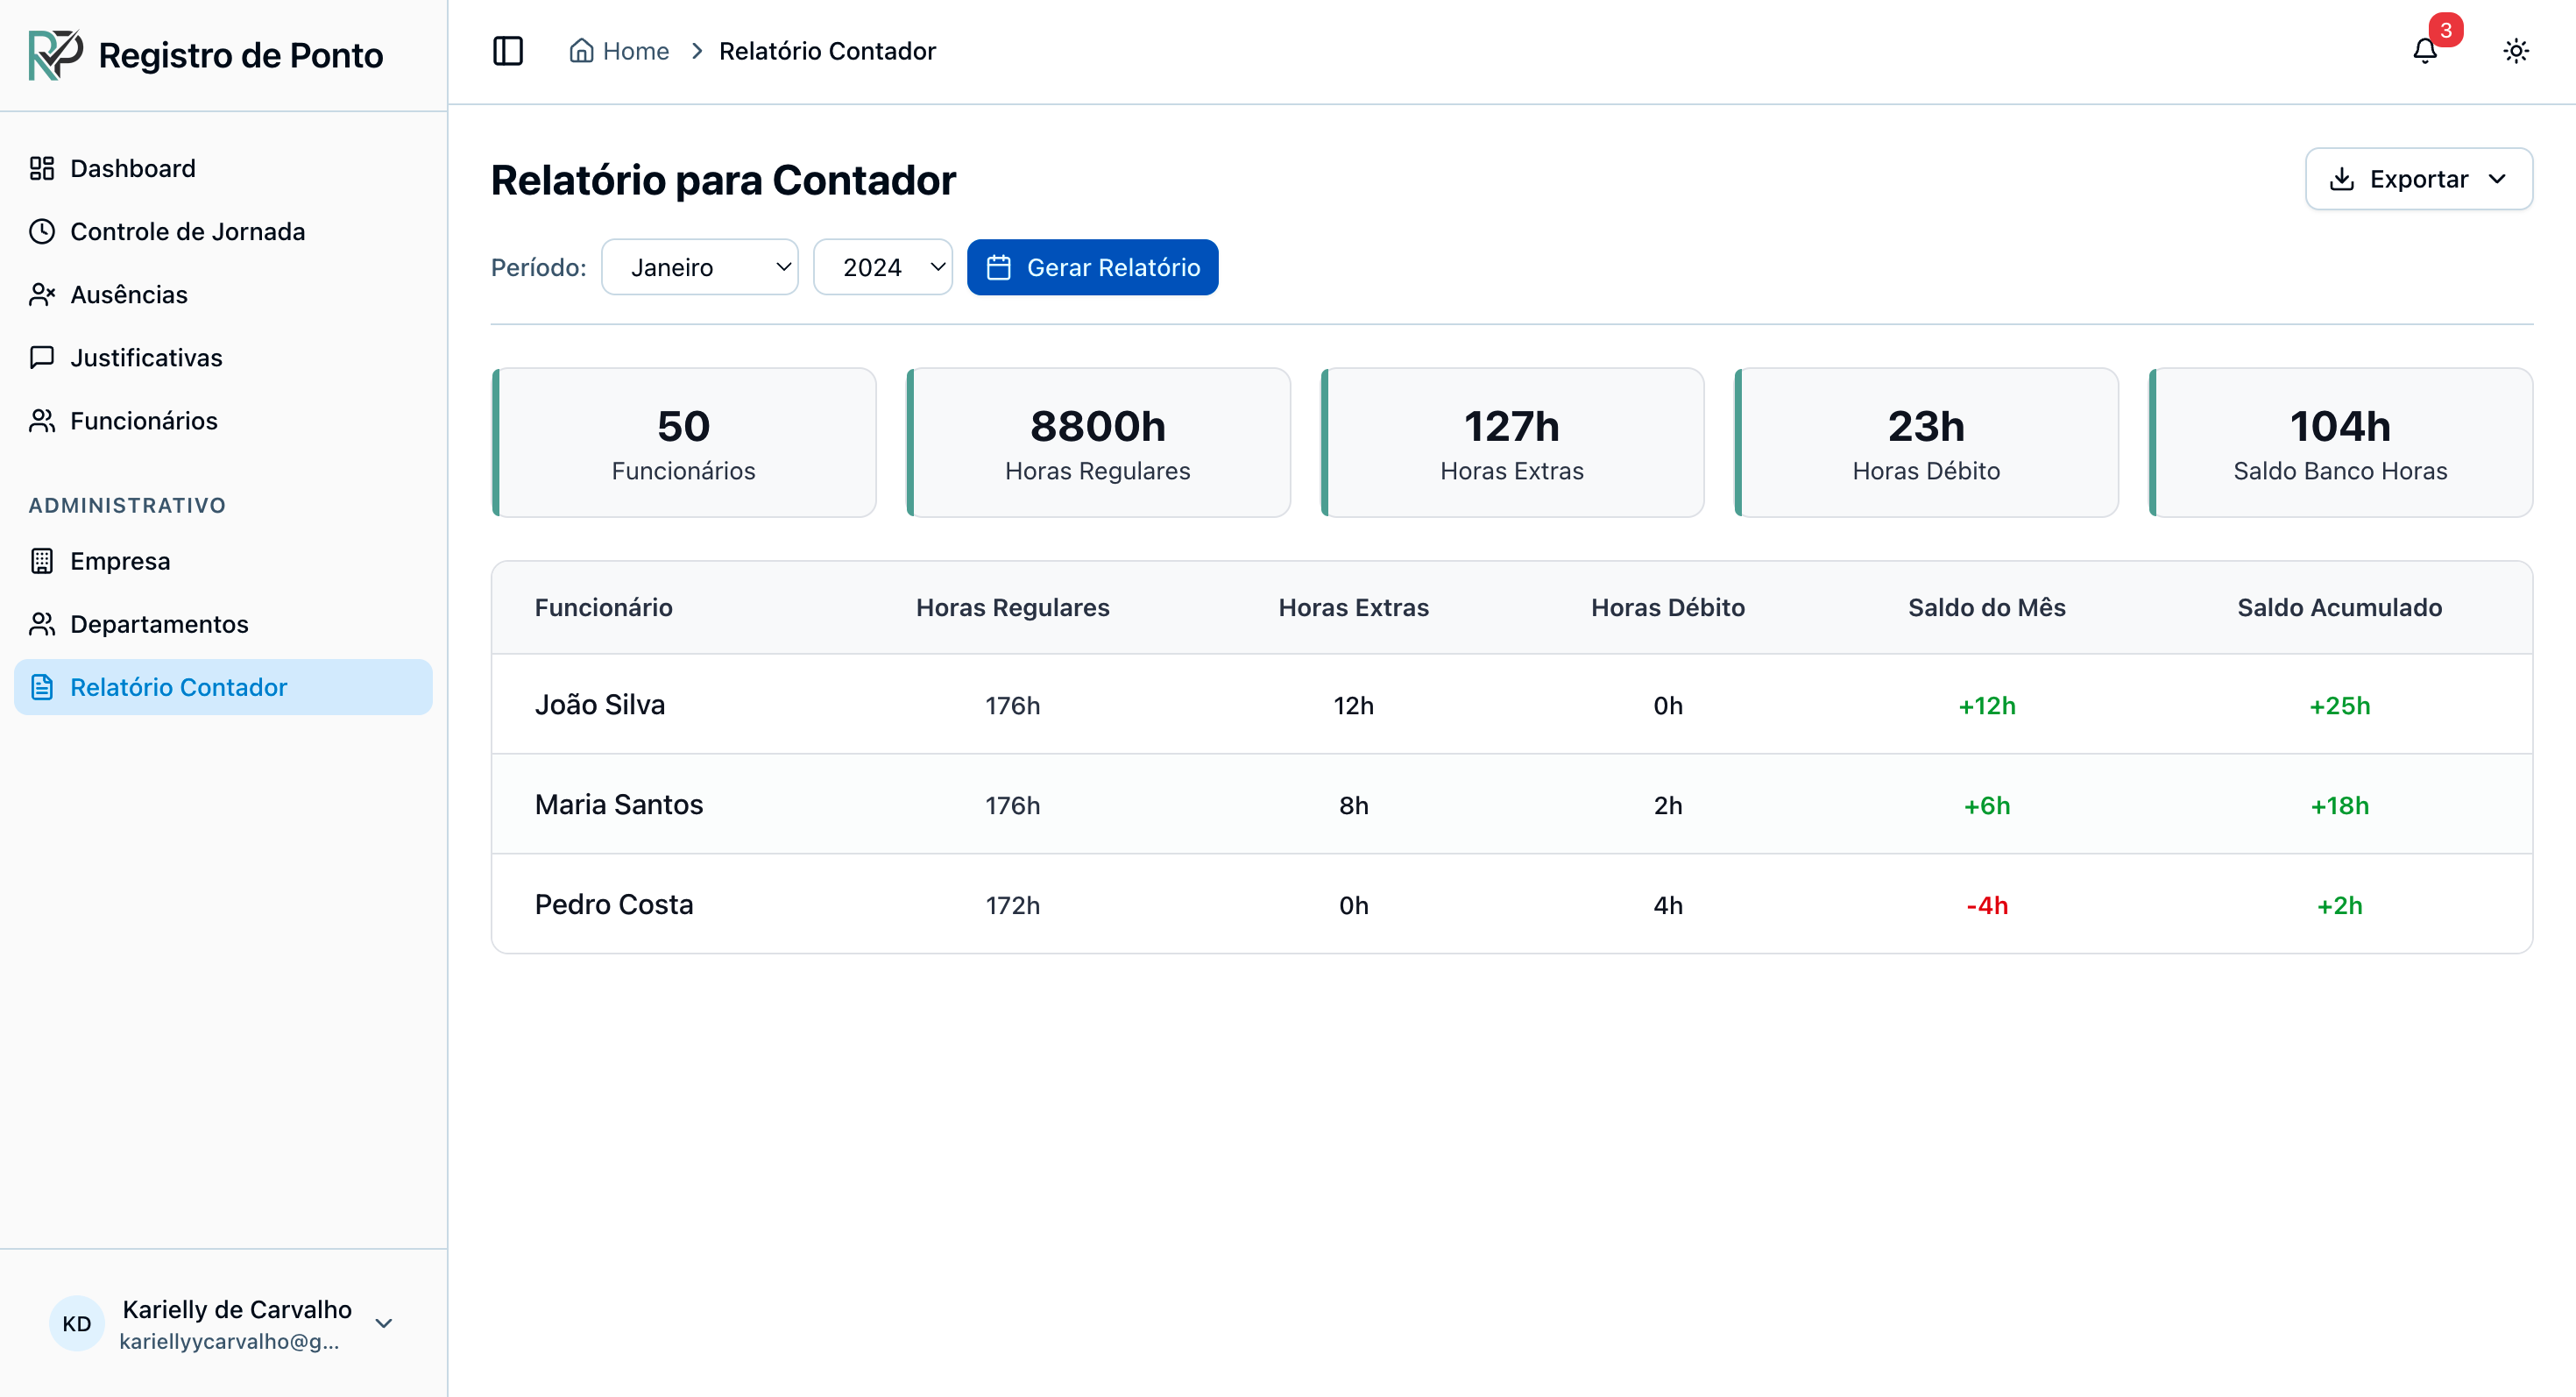
\includegraphics[width=0.7\textwidth]{imagens/relatorio-contador.png}
\caption{Relatório consolidado para contador}
\label{fig:relatorio-contador}
\end{figure}

Este relatório inclui:

\begin{itemize}
\item \textbf{Resumo Executivo}: Métricas gerais como total de funcionários, horas regulares, extras e banco de horas.
\item \textbf{Detalhamento Individual}: Tabela com dados individuais de cada funcionário.
\item \textbf{Exportação}: Múltiplos formatos (PDF, Excel, CSV) para integração com sistemas contábeis.
\item \textbf{Seleção de Período}: Filtros por mês e ano para relatórios históricos.
\end{itemize}

\section{Módulo de Configurações da Empresa}

O sistema disponibiliza uma interface completa para configuração de parâmetros empresariais, permitindo personalização de acordo com as necessidades específicas de cada organização.

\begin{figure}[H]
\centering
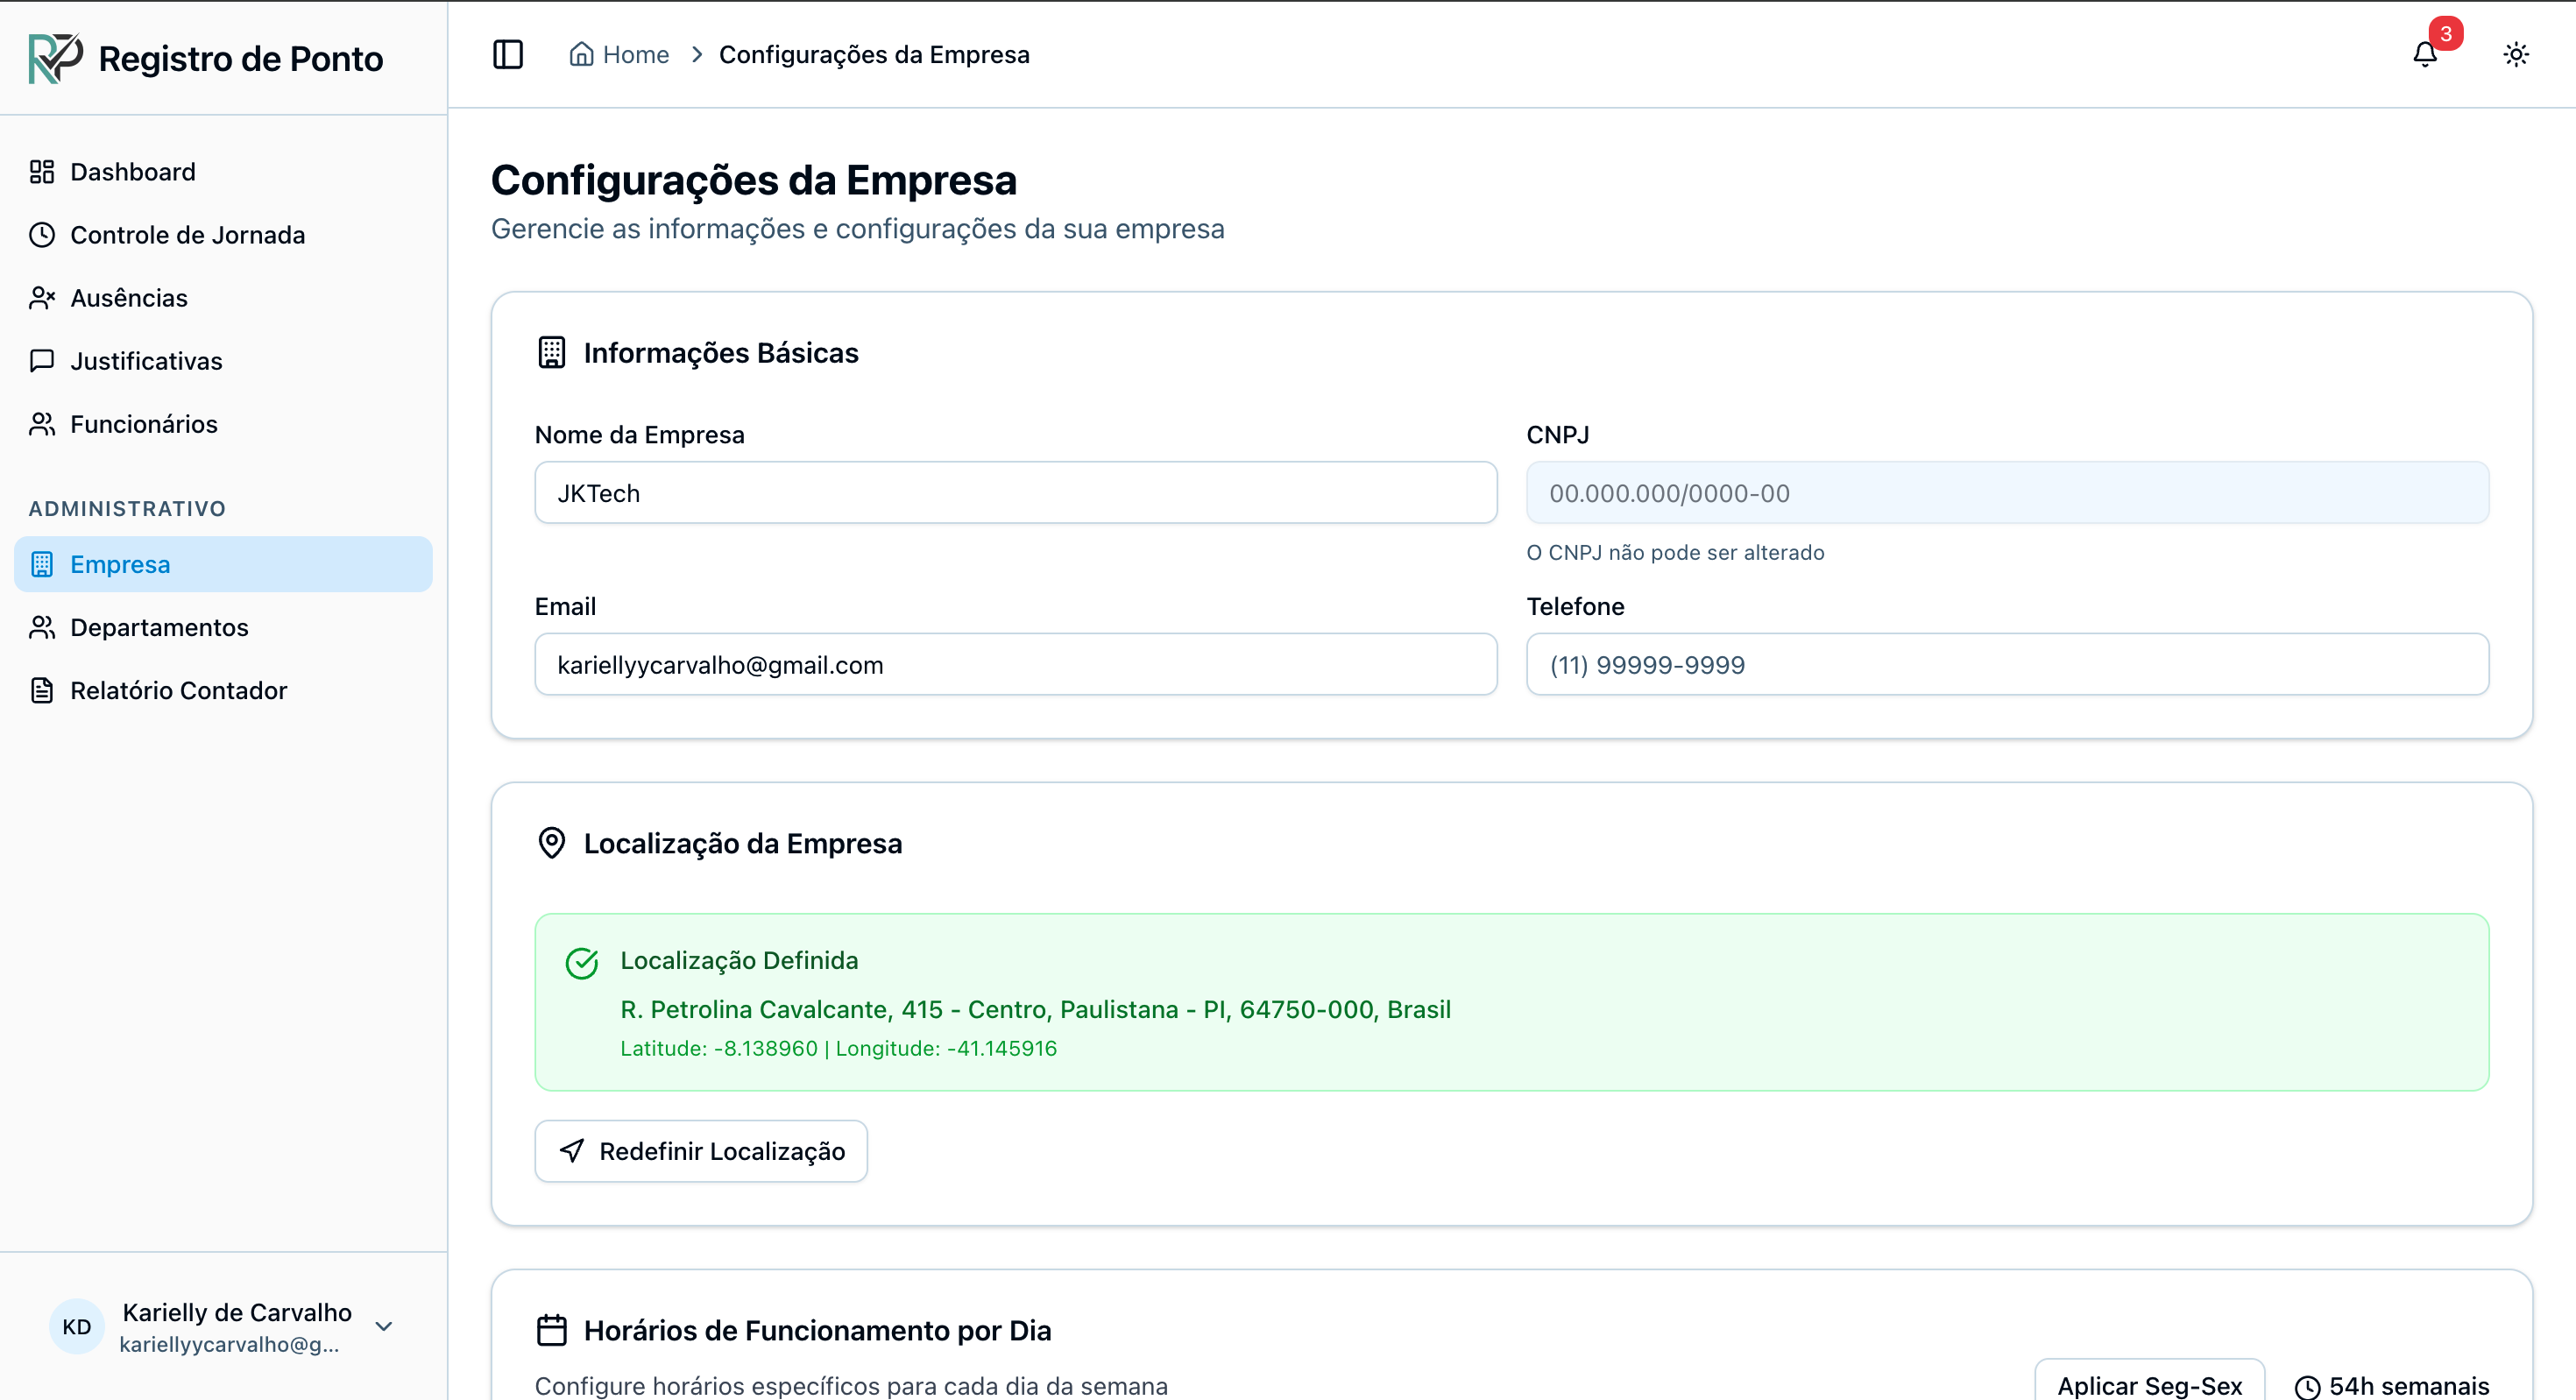
\includegraphics[width=0.7\textwidth]{imagens/configuracoes-empresa.png}
\caption{Configurações empresariais e parâmetros do sistema}
\label{fig:configuracoes-empresa}
\end{figure}

As configurações incluem:

\begin{itemize}
\item \textbf{Informações Básicas}: Nome, CNPJ, e-mail, telefone e endereço da empresa.
\item \textbf{Localização}: Configuração de coordenadas geográficas e raio permitido para registros.
\item \textbf{Horários de Funcionamento}: Definição de horários por dia da semana com intervalos.
\item \textbf{Tolerâncias}: Configuração de tolerâncias para entrada e saída.
\item \textbf{Políticas de Flexibilidade}: Regras para registros fora do raio da empresa.
\end{itemize}

\section{Interface de Registro de Ponto (Visão do Funcionário)}

Além da área administrativa, o sistema possui uma interface dedicada ao funcionário para o registro de seu ponto. Esta tela é projetada para ser simples e objetiva, exibindo a data e hora atuais e um botão para que o colaborador registre sua entrada ou saída. O sistema captura a geolocalização no momento do registro para verificação de conformidade.

\begin{figure}[H]
\centering
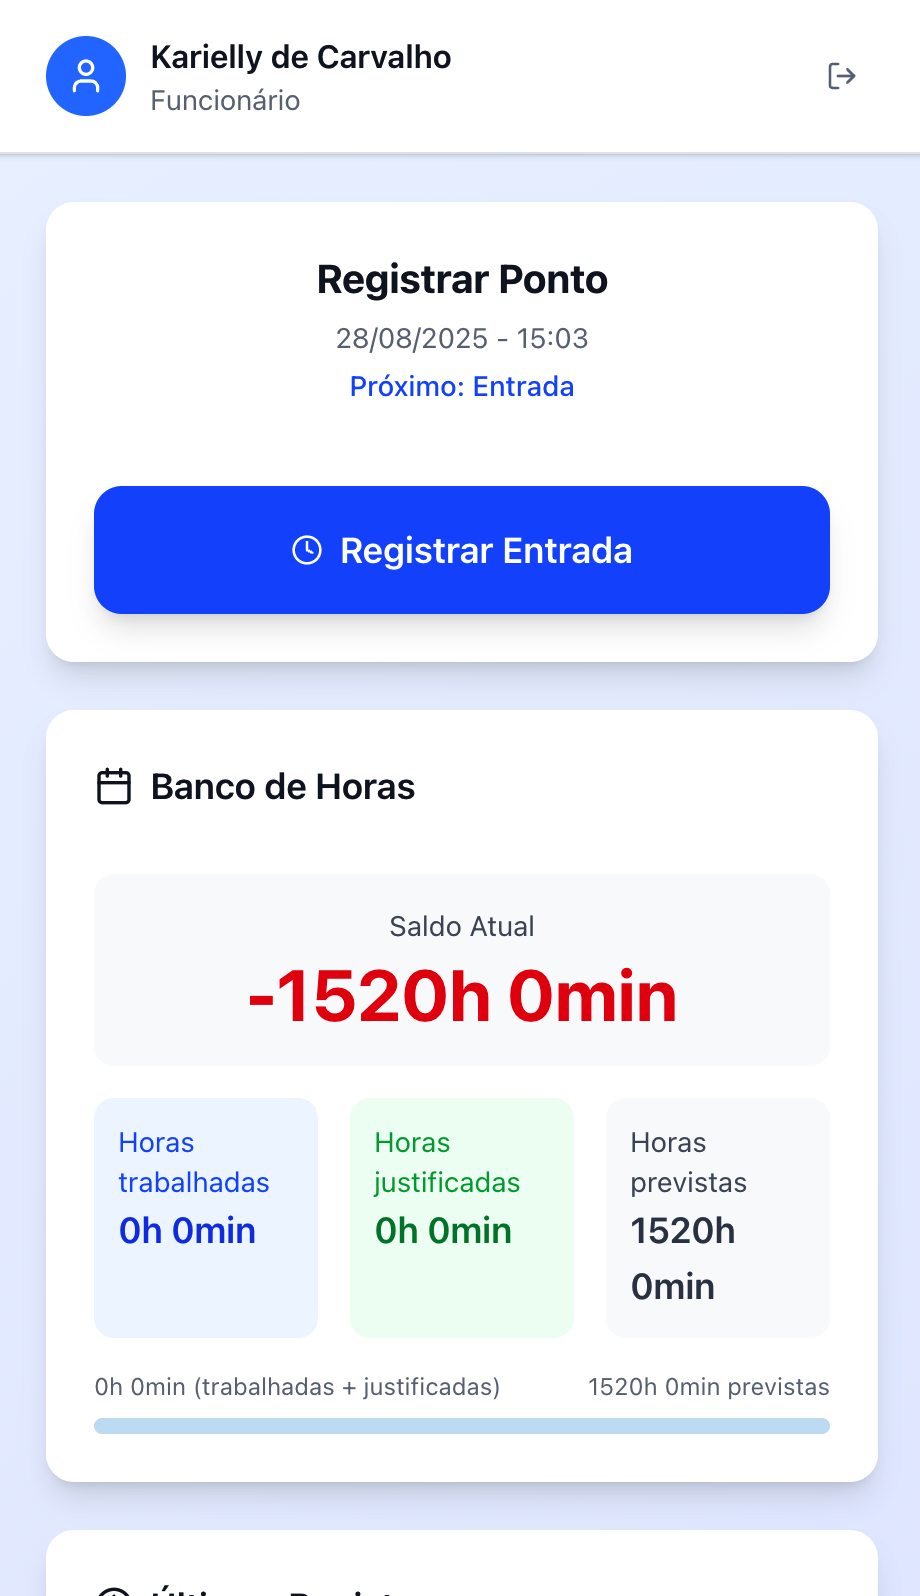
\includegraphics[width=0.35\textwidth]{imagens/registro-ponto-funcionario.png}
\caption{Interface de registro de ponto para funcionários}
\label{fig:registro-ponto-funcionario}
\end{figure}

\section{Personalização de Tema}

Para melhorar a experiência do usuário, o sistema oferece opções de personalização visual através do módulo de tema, permitindo alternância entre modos claro e escuro.

\begin{figure}[H]
\centering
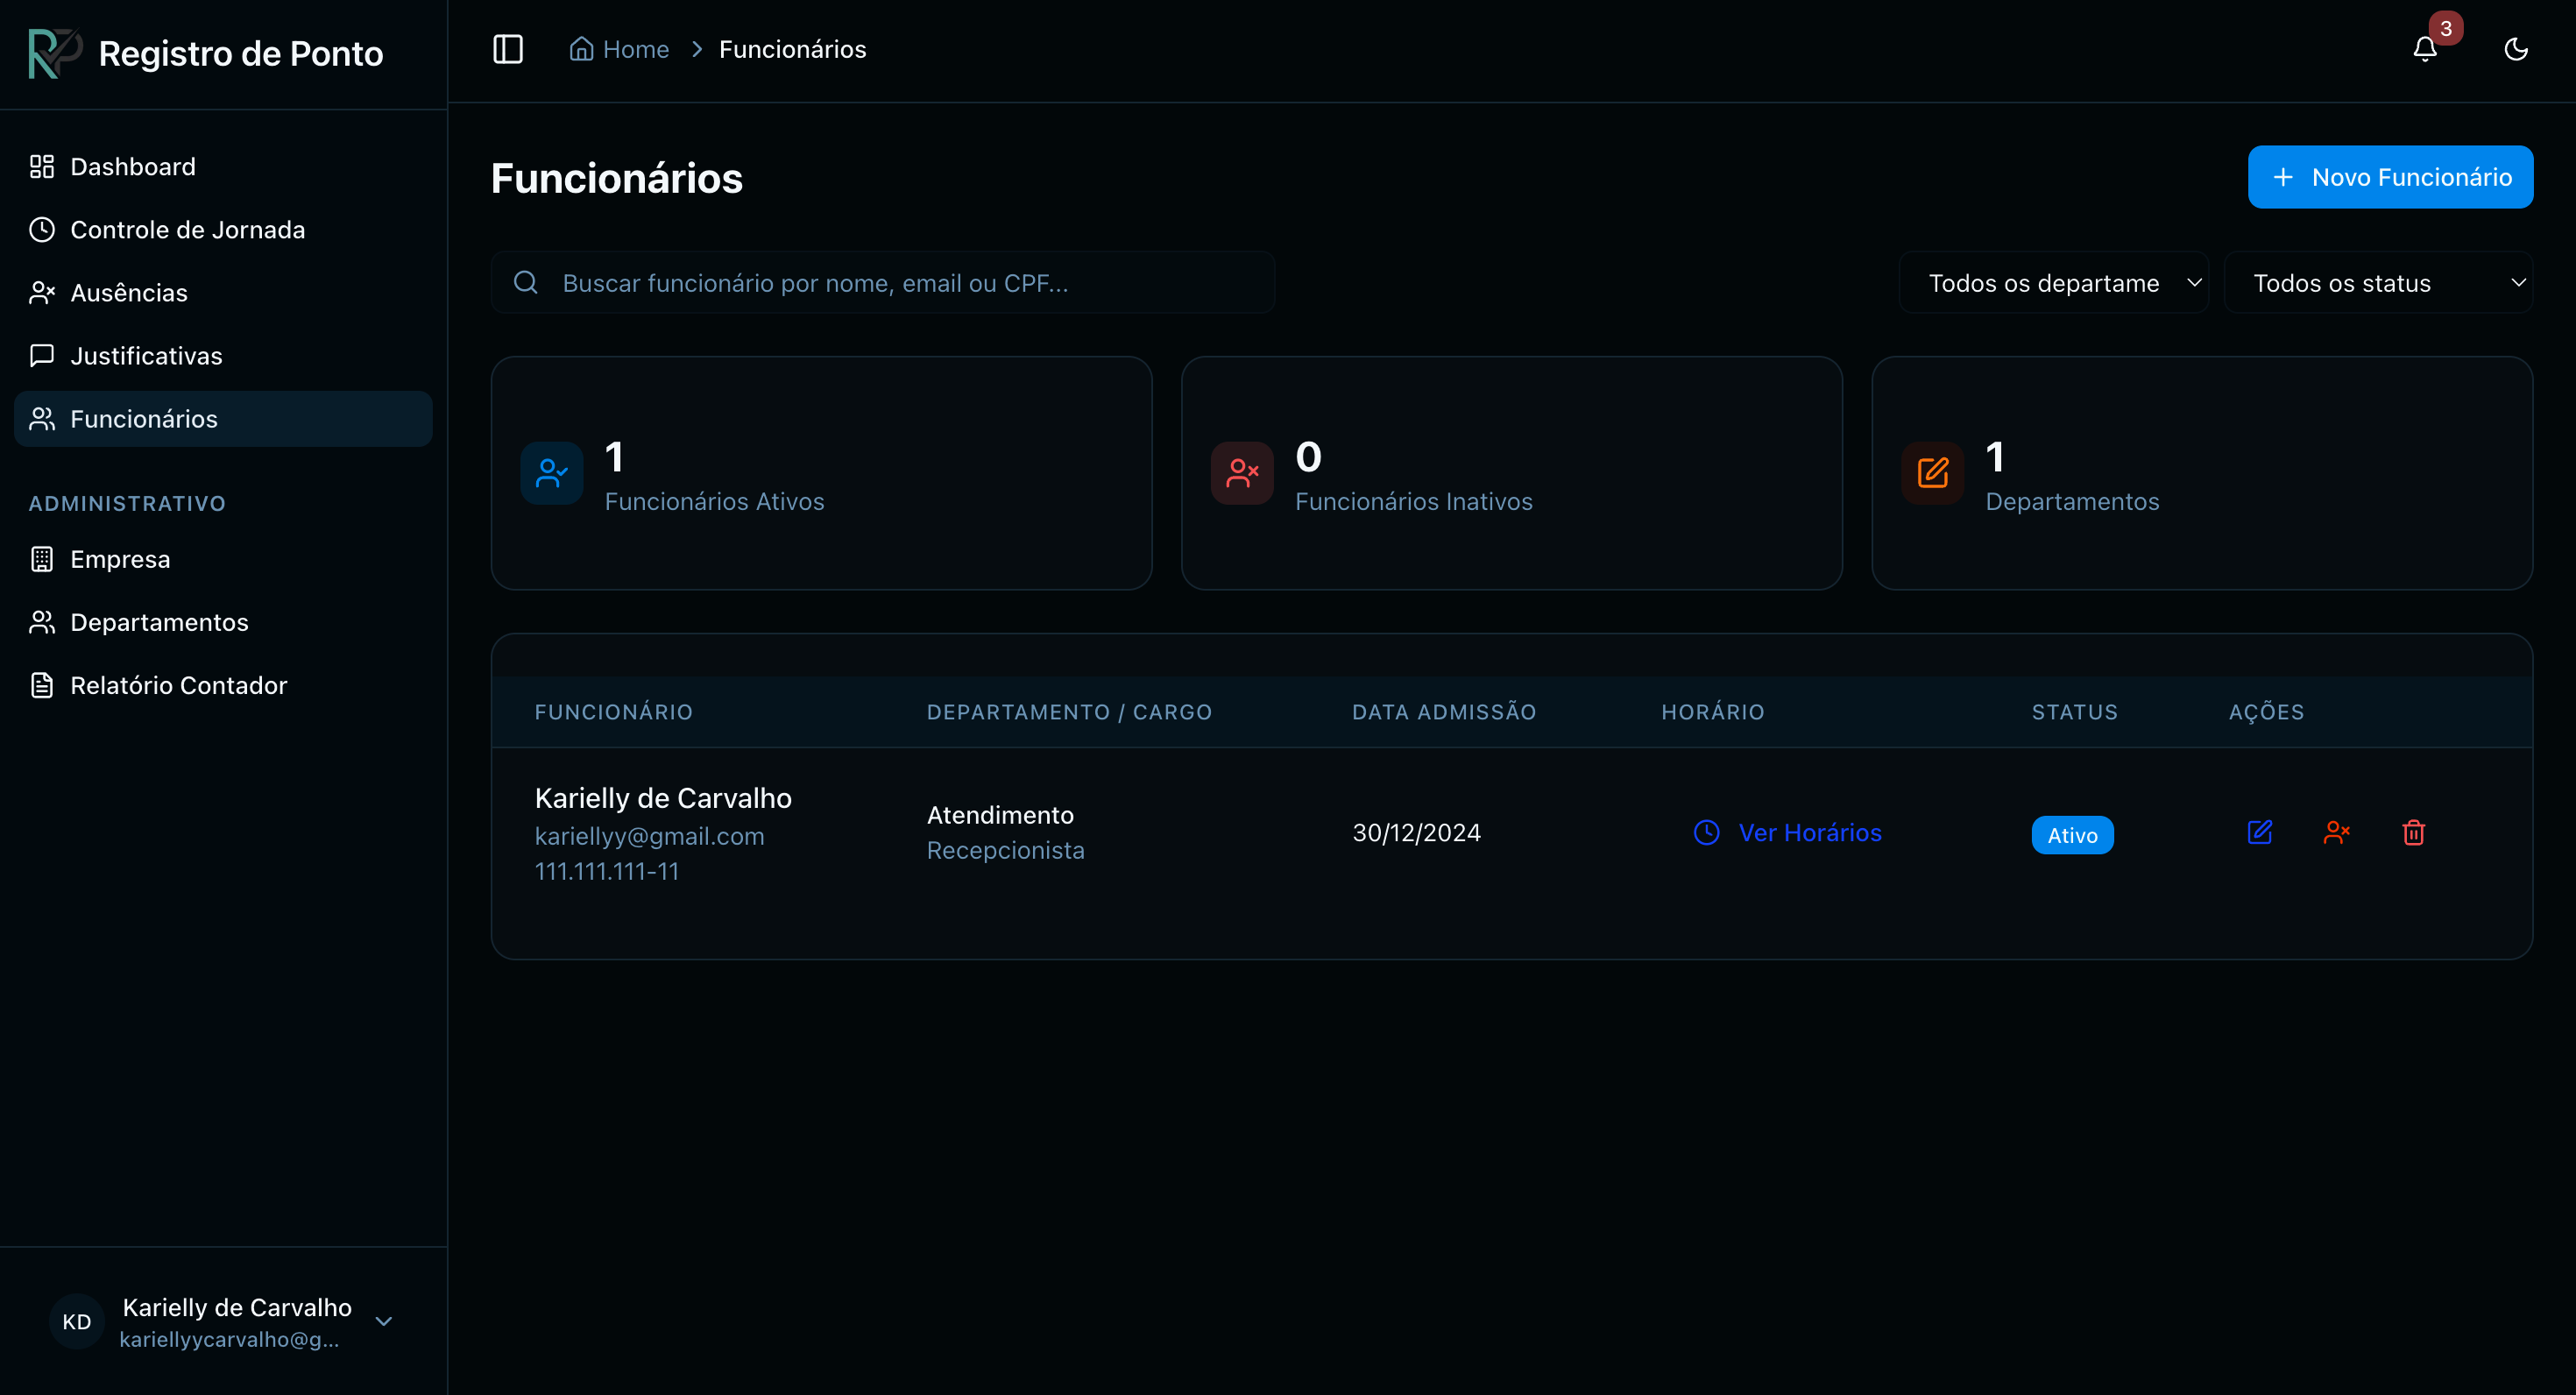
\includegraphics[width=0.6\textwidth]{imagens/configuracao-tema.png}
\caption{Opções de personalização de tema}
\label{fig:configuracao-tema}
\end{figure}

Este módulo permite:

\begin{itemize}
\item \textbf{Alternância de Tema}: Mudança entre modo claro e escuro.
\item \textbf{Prévia em Tempo Real}: Visualização imediata das alterações.
\item \textbf{Persistência}: Manutenção das preferências entre sessões.
\end{itemize}